\chapter{Industrial application examples}
\label{chap:ApplicationExamples}
%
\abstract{In this chapter, different examples are provided to apply the tool presented in this book. The MOOTuning software is used to analyze the temperature control in a Continuous Stirred Tank Heater (CSTH) in Section~\ref{sec:CSTH} using two a three cost functions. Also a Continuos Stirred Tank Reactor (CSTR) is considered for the control of the concentration of the product in an isothermal case in Section~\ref{sec:CSTRVandeVusse}}
%

%
\section{Continuous Stirred Tank Heater}
\label{sec:CSTH}
%
\subsection{Description of the process}
\label{sec:DescriptionCSTH}
%
The control of a \gls{csth} is a common task in industrial processes. In this section, the control of the temperature of the \gls{csth} will be solved as a \gls{moop} using a \gls{2dof} \gls{pid} controller. The diagram of the process is presented in %
\begin{figure}[b]
	\centering
	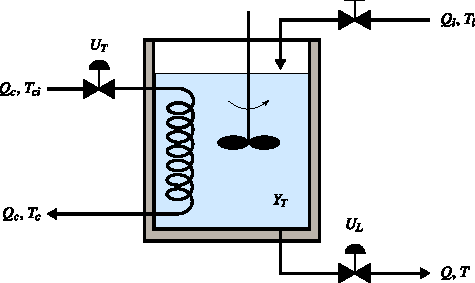
\includegraphics{Ch7CSTR}
	\caption{Simplified diagram of a continuous stirred-tank heater to be controlled.}
	\label{fig:Ch7CSTR}
\end{figure}
Figure~\ref{fig:Ch7CSTR}. A heat exchanger is installed inside the tank to heat the fluid. The flow rate inside the heat exchanger is controlled with a valve with input variable $U_T$ and the liquid inside the heat exchanger enters with temperature $T_{ci}$ and leaves with temperature $T_{co}$, the average temperature inide the heat exchanger is $T_{ca}$. The volume inside the tank is variable, the input flow rate is $Q_i$ with temperature $T_i$. The output flow rate is $Q$ with temperature $T$. The output flow rate is controlled with a valve with input variable $U_L$. The tank is covered with a jacket that prevents any heat loss to the atmosphere.

According to \citet{Alfaro2016}, a possible model for this process is given by the following set of algebraic-differential equations:
\begin{itemize}
	\item Tank mass balance:
			\begin{equation*}
				A \frac{d H(t)}{dt} = Q_i(t) - Q(t),
			\end{equation*}
			where $A$ is the transversal area of the tank and $H(t)$ is the liquid level.
	\item Tank energy balance:
			\begin{equation*}
				\rho C_p A H(t) \frac{T(t)}{dt} = \rho C_p Q_i(t)\left( T_i(t) - T(t)\right) + W(t),
			\end{equation*}
			where $C_p$ is the heat capacity of the fluid and $W(t)$ is the rate of heat transfer from the heat exchanger to the tank. $W(t)$ can be modeled as:
	\item Heat exchanger energy balance:
			\begin{equation*}
				\rho_c C_{pc} V_c \frac{T_{ca}(t)}{dt} = \rho_c C_{pc} Q_c(t)\left( T_{ci}(t)-T_{co}(t)\right) - W(t),
			\end{equation*}
			where $\rho_c$ is the density of the fluid inside the heat exchanger, $C_{pc}$ is the heat capacity of the fluid inside the heat exchanger and $V_c$ is the volume of the heat exchanger.
	\item Heat transfer between the heat exchanger and the fluid in the tank:
			\begin{equation*}
				W(t) = U A_c \left( T_{ca}(t) - T(t)\right), 
			\end{equation*}
			where $U$ is overall heat-transfer coefficient, $A_c$ is the area of the heat exchanger, $T_{ca}(t)$ is the average temperature inside the heat exchanger which is related to $T_{co}(t)$ and $T_{ci}(t)$ as:
			\begin{equation*}
				T_{ca}(t) = \frac{T_{ci}(t) + T_{co}(t)}{2}
			\end{equation*}
\end{itemize}

Also, in \citet{Alfaro2016}, the transmitters and the valves are modeled as:
\begin{itemize}
	\item Level transmitter: it is supposed that the level transmitter is a capacitive type electronic transmitter that has a first order dynamics:
		\begin{equation*}
			T_L \frac{d Y_L(t)}{dt} + Y_L(t) = K_L H(t),
		\end{equation*}
		%
		where $T_L$ is its time constant, $Y_L$ is the level signal and $K_L$ is the transmitter gain.
	%
	\item Temperature transmitter: It is supposed that a Pt$_{100}$ RTD electronic sensor is installed in a thermowell at the tank outlet pipe. It is supposed that it has a second order dynamic:
	%
		\begin{equation*}
			T_{T}^2 \frac{d^2 Y_T(t)}{dt^2} + 2T_T \frac{d Y_T(t)}{dt} + Y_T(t) = K_T T(t),
		\end{equation*}
		%
		where $T_T$ is its time constant and $K_T$ is its gain.
	%
	\item Level control valve: it is supposed that a ball valve with an electroneumatic actuator is used. The valve	inherent flow characteristics is nearly quadratic and the relationship between the flow $Q(t)$ and the input variable $U_L$ is given by:
		\begin{align*}
			T_{vL} \frac{d X_L(t)}{dt} + X_L(t) = K_{xL} U_L(t),\\
			Q(t) = K_{vL} X_L^2(t)\sqrt{\rho g H(t)},
		\end{align*}
		where $T_{vL}$ is the level control valve time constant, $K_{xL}$ level control valve stem constant $K_{vL}$ level control valve constant and $X_L(t)$ is the level control valve stem normalized travel.
	%
	\item Temperature control valve it is also supposed to be a ball valve with an electroneumatic actuator, however, it is supposed that the valve has an equal-percentage inherent flow characteristics given by:
		\begin{align*}
			T_{vT} \frac{d X_T(t)}{dt} + X_T(t) = K_{xT} U_T(t),\\
			Q_c(t) = K_{vT}R_{vT}^{\left( X_T(t) -1 \right) } \sqrt{P_{cp} - \left(R_c Q^2_c(t)+P_{cr} \right) },
		\end{align*}
		where $T_{vT}$ is the temperature control valve time constant, $K_{xT}$ the temperature control valve stem constant, $K_{vT}$ is the temperature control valve constant $P_{cp}$ is the heating fluid pump discharge pressure, $P_{cr}$ is heating fluid system return pressure and $X_T(t)$ is the temperature control valve stem normalized travel.
\end{itemize}

Taking this model in consideration, it can be said that, from the point of view of the controller, the controlled variables are give by the signals $Y_L(t)$ (which represents the level) and $Y_T(t)$ (which represents the temperature of the fluid of the tank). The manipulated variables are given by $U_L(t)$ (which directly affects $Q$) and $U_T(t)$ (that directly affects $Q_{c}$). $Q_i(t)$, $T_i$ and $T_{ci}$ are considered as disturbances. The state variables of the system are given by $H(t)$, $T_T(t)$, $T_{co}$, $Y_L(t)$, $Y_T$, $X_L(t)$ and $X_T(t)$, therefore, this model comprises a seventh order non-linear system for a two-input two-output industrial process. The parameters of the model can be found in 
\begin{table}
	\centering
	\caption{Parameters for the CSTH process}
	\label{tab:ParametersCSTH}
	\begin{tabular}{ccc}
		\toprule
		\textbf{Symbol} & \textbf{Value} & \textbf{Description}\\
		\midrule
		\multicolumn{3}{c}{\textbf{\textit{Tank parameters}}}\\
		\midrule
		$\rho$ 		& \SI{1200}{\kilogram\per\meter\cubed} 			& tank fluid density\\
		$A$			& \SI{0.0707}{\square\meter}					& tank inside section area\\
		$C_p$		& \SI{4190}{\joule\per\kilogram\per\celsius}	& tank fluid heat capacity\\
		$g$			& \SI{9.8}{\meter\per\square\second}			& gravity acceleration\\
		$K_T$		& \SI{2}{\%\per\celsius}						& temperature transmitter gain\\
		$K_{vL}$	& \num{1.25e-5}									& level control valve constant\\
		$K_{vT}$	& \num{3e-6}									& temperature control valve constant\\
		$K_{xL}$	& \SI{0.01}{\per\%}								& level control valve stem constant\\
		$Q_i$		& \SI{7e-4}{\cubic\meter\per\second}			& normal tank inlet fluid flow rate\\
		$T_i$		& \SI{24}{\celsius}								& fluid inlet temperature\\
		$T_L$		& \SI{2}{\second}								& level transmitter time constant\\
		$T_T$		& \SI{15}{\second}								& temperature transmitter time constant\\
		$T_{vL}$	& \SI{3}{\second}								& level control valve time constant\\
		$T_{vT}$	& \SI{5}{\second}								& temperature control valve time constant\\
		\midrule
		\multicolumn{3}{c}{\textbf{\textit{Heat exchanger parameters}}}\\
		\midrule
		$\rho_c$ 	& \SI{800}{\kilogram\per\meter\cubed} 			& heating fluid density\\
		$A_c$		& \SI{0.6362}{\square\meter}					& heat exchanger transfer area\\
		$C_{pc}$	& \SI{2400}{\joule\per\kilogram\per\celsius}	& heating fluid heat capacity\\
		$K_L$		& \SI{125}{\%\per\meter}						& level transmitter gain\\
		$K_{xT}$	& \SI{0.01}{\per\%}								& temperature control valve stem constant\\
		$P_{cp}$	& \SI{4.14e5}{\pascal}							& heating fluid pump discharge pressure\\
		$P_{cr}$	& \SI{1.38e5}{\pascal}							& heating fluid system return pressure\\
		$R_c$		& \SI{5.5e10}{\pascal\per(\cubic\meter\per\second)^2}	& heating system pipe nominal flow resistance\\
		$R_{vT}$	& \num{50}										& temperature control valve rangeability\\
		$T_{ci}$	& \SI{320}{\celsius}							& heating fluid inlet temperature\\
		$U$			& \SI{440}{\joule\per\second\per\square\meter\per\celsius}	& overall heat-transfer coefficient\\
		$V_c$		& \SI{0.0139}{\cubic\meter}						& heat exchanger volume\\
		\bottomrule
	\end{tabular}
\end{table}
%
Table~\ref{tab:ParametersCSTH}. This model was implemented in \simulink and can be found with the companion software. In %
%
\begin{figure}[tb]
	\centering
	\includegraphics[width=\columnwidth]{Ch7Implementation}
	\caption{\simulink implementation of the model of the heater.}
	\label{fig:Ch7Implementation}
\end{figure}
%
Figure~\ref{fig:Ch7Implementation}. Each equation of the model was implemented in a subsystem for clarity. For example in %
\begin{figure}
	\centering
	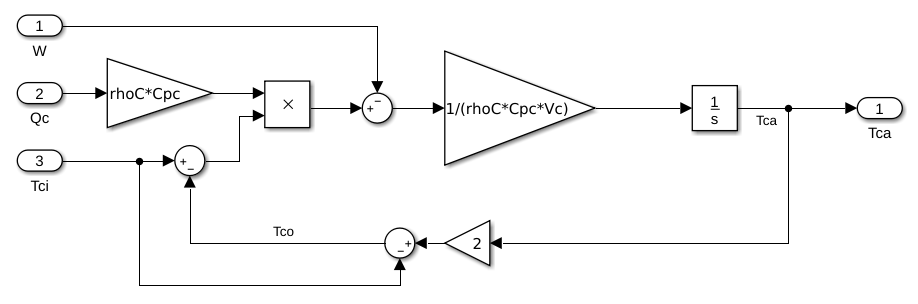
\includegraphics[width=\columnwidth]{Ch7HeatExhangerEq}
	\caption{Example of the implementation of the heat exchanger energy balance.}
	\label{fig:Ch7HeatExhangerEq}
\end{figure}
%
Figure~\ref{fig:Ch7HeatExhangerEq} the \simulink implementation of the heat exchanger energy balance is presented. The result of this submodel is the computation of the state variable $T_{ca}$, which represents the average temperature of the heating fluid. As it can be seen, the parameters of the model are not hard-coded in the \simulink blocks, instead a parameter initialization script is call before the simulation starts. If the user desires to change any value of the parameters, it can be done globally in the script and then automatically called during the simulation.

\subsection{Simplified linear model}
\label{sec:SimpLinMod}
In order to find a PID controller using the MOOTuning app, it is necessary to find a linear model of the plant in the operation point. An identification procedure was performed with a change of 10\% in the value of $U_T$ to find the transfer function between $Y_T$ and $U_T$. The response to this change is depicted in %
\begin{figure}[tb]
	\centering
	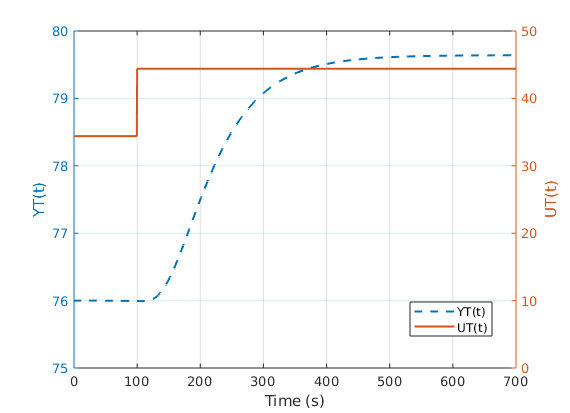
\includegraphics[width=\columnwidth]{Ch7CSTHResp}
	\caption{Response of the process to a change of 10\% in the $U_T(t)$ input.}
	\label{fig:Ch7CSTHResp}
\end{figure}
%
Figure~\ref{fig:Ch7CSTHResp}. As it can be seen, the response is overdamped and takes approximately \SI{500}{\second} to reach a new steady state. A change in 10\% on the input signal produces a variation of approximately $3.5\%$ in the output signal. It has to be noticed that the presented signals are normalized between 0 and 100\% representing the full spam of the transmitter and actuators.

In order to find the model, the process was supposed to have two poles, no zeros and a pure time-delay (also known as dead-time). Of course, if a linearization procedure were performed using the nonlinear model, a seventh order model would be obtained. However, for PID tuning, a first or second order model is usually expected to tune the controller.

Considering the experiment performed with the data as depicted in Figure~\ref{fig:Ch7CSTHResp}, the resulting simplified model is given by:
%
\begin{equation}
\frac{Y_T(s)}{U_T(s)} = \frac{0.3658 e^{-24.736 s}}{(52.861 s+1)(52.805 s +1)}.
\label{eq:TFCSTH}
\end{equation}

From this transfer function, it can be deduced that the gain is equal to $K = 0.3658$, the main time constant is given by $T = 52.861$, the ratio between the two time constant is given by $a = 0.9989$ and the dead-time is given by $L = 24.736$, therefore the normalized dead-time is given by $\tau = 0.4679$.

To test the validity of this simplified model, the response of the transfer function is compared against the response of the non-linear model. It was found that the transfer function response is very similar to the response of the non-linear model, as can be seen in %
%
\begin{figure}[tb]
	\centering
	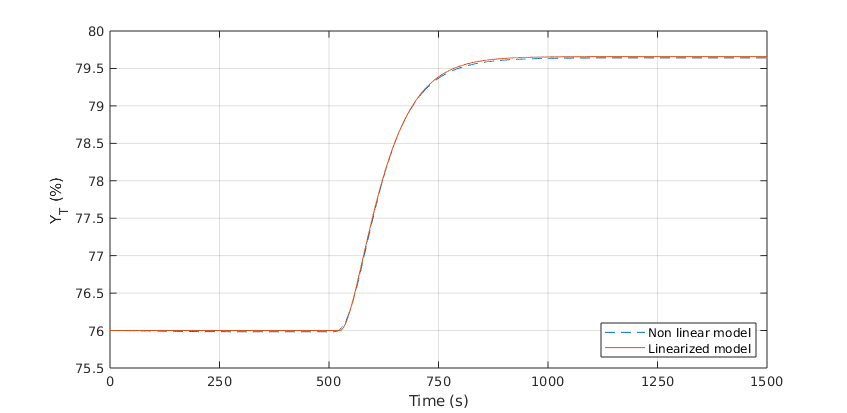
\includegraphics[width=\columnwidth]{Ch7CSTHComp}
	\caption{Comparison between the linear and no linear models for the CSTH.}
	\label{fig:Ch7CSTHComp}
\end{figure}
%
Figure~\ref{fig:Ch7CSTHComp}. It is clear that the non-linear model is a good representation of the dynamical response of the process. This is the first step in order to find a suitable PID controller to control the plant. In \citet{Alfaro2016} the level of the tank is also controlled, however the dynamic of the level is simpler (its model can be approximated with a first order model without delay) and in this particular example, only the temperature is going to be controlled, while the level is considered to be constant.
%
\subsection{PID control of the CSTH considering two integral cost functions}
\label{sec:PIDCSTH}
In this section, the process will be controlled using a \gls{pid} controller with different tuning methods and compared with the \gls{moo} framework used in the book.

Two different tuning rules were considered: the method by \citet{Rovira1969a} and the method by \citet{Murril1967}. For the case of the Rovira and Murril method, the model in \eqref{eq:TFCSTH} was reduced to a first order model using the Half-Rule in \citet{Skogestad2003}:
\begin{equation}
\frac{Y_T(s)}{U_T(s)} = \frac{0.3658 e^{-24.7360 s}}{79.2635 s +1}.
\label{eq:TFCSTHFirstOrder}
\end{equation}

The equations were implemented as presented in \citet{odwyer2006}:
\begin{itemize}
%	\item SIMC method: Supposing a \gls{soptd} model:
%			\begin{equation*}
%				P(s) = \frac{K e^{-Ls}}{(Ts+1)(aTs+1)}
%			\end{equation*}
%			The corresponding PID tuning for a closed-loop lag time of $T_c = L$ and the case where $T \leq 8 L$, the PID tuning is given by:
%			\begin{align*}
%				K_p &= \frac{0.5}{K}\frac{(1+a)T}{L}\\
%				T_i &= (1 + a) T\\
%				T_d	&= \frac{a}{1+a}T
%			\end{align*}
%	%
	\item Supposing a \gls{foptd} model given by:
			\begin{equation*}
				P(s) = \frac{K e^{-L s}}{Ts+1}
			\end{equation*}
			The Murrill tuning is given by:
				\begin{align*}
					K_p &= \frac{1.435}{K}\left( \frac{T}{L} \right)^{0.921}\\
					T_i &= \frac{T}{0.878}\left( \frac{L}{T}\right)^{0.749}\\\\
					T_d &= 0.482 T \left( \frac{L}{T} \right)^{1.137}
				\end{align*}
	\item Again, supposing a \gls{foptd} as above, the Rovira tuning is given by:
			\begin{align*}
				K_p &= \frac{1.086}{K} \left( \frac{T}{L}\right) ^{0.869} \\
				T_i &= \frac{T}{0.740 - 0.13\frac{L}{T}} \\
				T_d &= 0.384 T \left( \frac{L}{T}\right)^{0.914} 
			\end{align*}
\end{itemize}

The values of the computed values can be found on %
\begin{table}[tb]
	\centering
	\caption{Comparison of different PID tunings for the CSTH process.}
	\setlength{\tabcolsep}{8pt}
	\begin{tabular}{ccccccc}
		\toprule
		Tuning 	& $K_p$ 	& $T_i$		& $T_d$		& $\beta$	& $J_{r}$	& $J_{di}$\\
		\midrule
		%
		%SIMC	& $5.84$	& $105.67$	& $26.42$	& $1$			& $55.14$	& $18.10$\\
		Murril	& $5.87$	& $65.02$	& $23.21$	& $1$			& $82.51$	& $15.34$\\
		Rovira	& $4.34$	& $120.81$	& $18.48$	& $1$			& $76.00$	& $27.79$\\
		MOO01	& $11.3$	& $58.82$	& $29.48$	& $0.43$		& $85.65$	& $7.06$\\
		MOO02	& $9.26$	& $123.85$	& $26.68$	& $0.80$		& $69.96$	& $13.38$\\
		MOO03	& $8.20$	& $185.21$	& $28.14$	& $0.99$		& $67.93$	& $22.54$\\
		\bottomrule
	\end{tabular}
	\label{tab:CompPIDCSTH}
\end{table}
%
Table~\ref{tab:CompPIDCSTH}, along with its associated values of $J_{di}$ and $J_r$. The Murril and Rovira methods presented in the table were selected because they are intended to minimize the \gls{iae}. In all cases, the PID tuning is for a one degree of freedom controller (that is  the reason why $\beta$ is equal to one).

The PID that can be found using the data and the framework presented in Chapter~\ref{chap:PIDMOOP} is a \gls{soptd}, which may do the comparison somehow unfair. However, the idea now is to compare methods that tries to minimize the \gls{iae}. Using the MOOTuning Tool that accompanies this book, the Pareto front that was found is given as in %
%
\begin{figure}[tb]
	\centering
	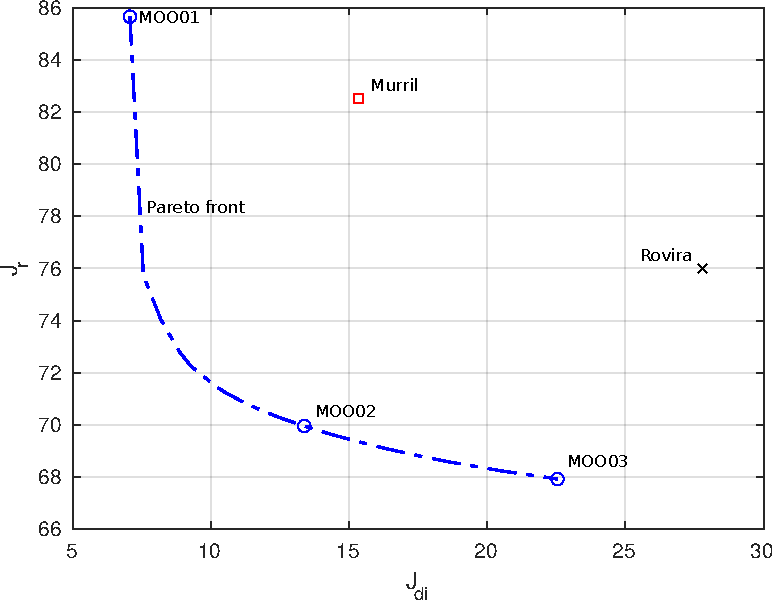
\includegraphics[width=\columnwidth]{Ch7CompPareto}
	\caption{MOOTuning compared to the Murril and Rovira methods that also minimizes \gls{iae}.}
	\label{fig:Ch7CompPareto}
\end{figure}
%
Figure~\ref{fig:Ch7CompPareto}. As it was expected, all the controllers found using the \gls{moo} tool present lower values for $J_{di}$ and $J_r$. If all controllers had the same topology, most certainly both controller would be close to the anchor points. However, what it is important here is the fact that, using the tool, the user has the ability to chose between practically an infinity of possible controllers. From the Pareto front, three different tuning were selected in order to compare the responses using the non-linear plant. The values of the parameters are presented also in Table~\ref{tab:CompPIDCSTH} and depicted as circles in the Pareto front in Figure~\ref{fig:Ch7CompPareto}.
%
\begin{figure}[tb]
	\centering
	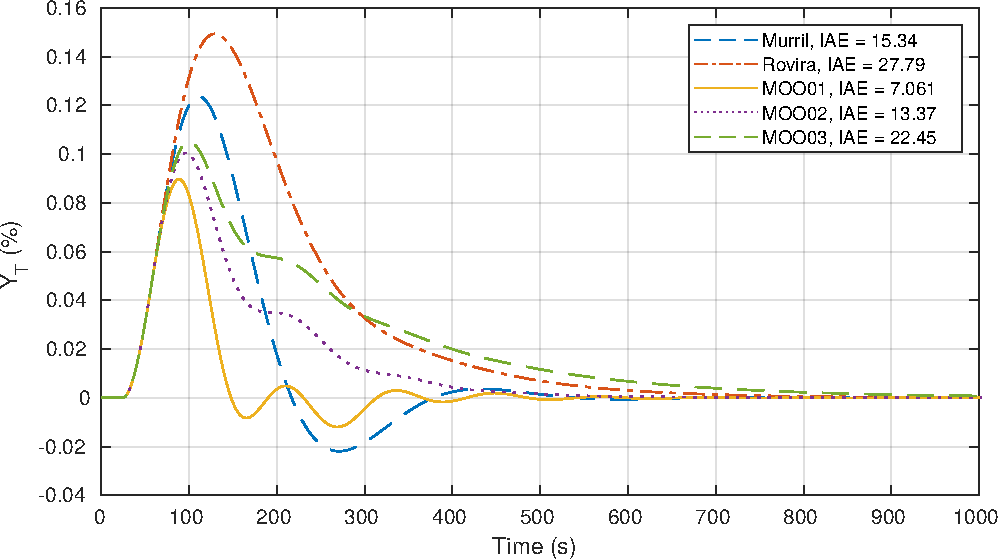
\includegraphics[width=\columnwidth]{Ch7CompParetoReg}
	\caption{Regulator response comparison for minimum IAE.}
	\label{fig:Ch7CompParetoReg}
\end{figure}
%
\begin{figure}[tb]
	\centering
	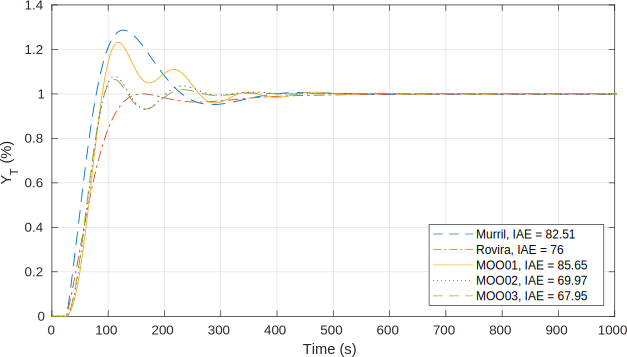
\includegraphics[width=\columnwidth]{Ch7CompParetoServo}
	\caption{Servo response comparison for minimum IAE.}
	\label{fig:Ch7CompParetoServo}
\end{figure}

In Figures~\ref{fig:Ch7CompParetoReg} and \ref{fig:Ch7CompParetoServo} the responses to a step change in the setpoint and in the disturbance are presented. The corresponding values of \gls{iae} are also presented in the graph. In all cases, the robustness was not considered as a constraint. but it is possible to include it within the MOOTuning software. From Figure~\ref{fig:Ch7CompPareto} given the steep slope of the curve for lower values of $J_{di}$ that a small change in $J_{di}$ may improve substantially the performance for $J_r$. Therefore, one may be more prone to select a controller that may have a little degradation in $J_{di}$ and for this reason, controller MOO01 may not be a good selection as a final solution unless having the minimum value possible of $J_{di}$ is the final goal.

The controller MOO02 may be seen as an intermediate solution between MOO1 and MOO03 in case both $J_{di}$ and $J_r$ are equally important for the decision maker. The power of the multiobjective framework is evident, and giving that the computational power is done offline, it becomes a good tool for the tuning of PIDs in an industrial setting.

To check how the tuning performs with the nonlinear model, a simulation was performed using the tuning of the controller $MOO02$. The setpoint was increased by $5\%$ at $t=\SI{100}{\second}$ and the temperature of the steam was increased by $\SI{10}{\celsius}$ at $t=\SI{700}{\second}$. The response is presented in %
\begin{figure}[tb]
	\centering
	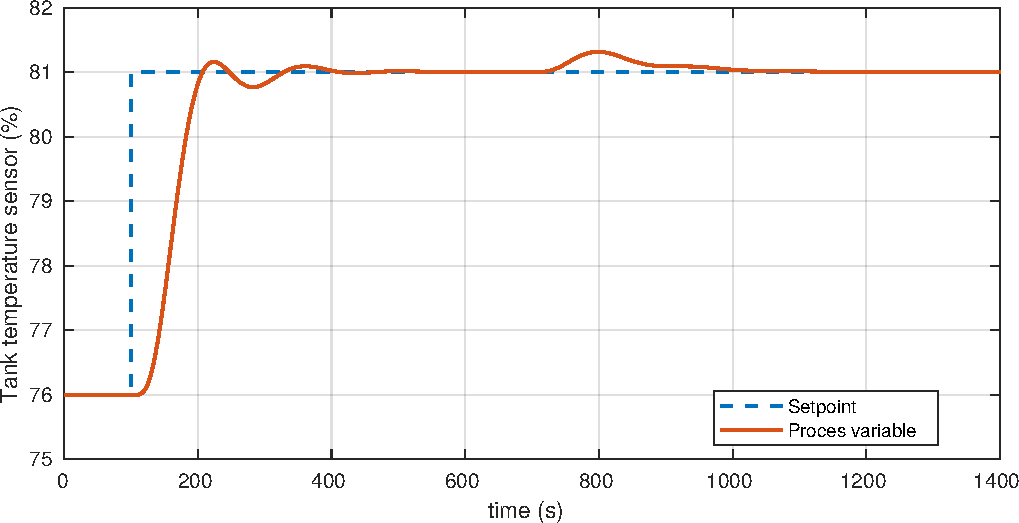
\includegraphics[width=\columnwidth]{Ch7CSTRControlled}
	\caption{Response of the controlled system using the nonlinear model for the CSTH.}
	\label{fig:Ch7CSTRControlled}
\end{figure}
%
Figure~\ref{fig:Ch7CSTRControlled}. As it can be seen, the servo response is very close to the one presented in Figure~\ref{fig:Ch7CompParetoServo}, which is a clear indicator that the linear model was a good approximation of the plant at the given operation point. The response to the change in the stem temperature cannot be compared with the regulation presented in Figure~\ref{fig:Ch7CompParetoReg}, because the disturbance was not applied directly in the input of the plant. However, it is interesting to note that the controller was able to respond with a good dynamic even though it was not optimize for this case.

The controlled variable is presented in %
\begin{figure}[tb]
	\centering
	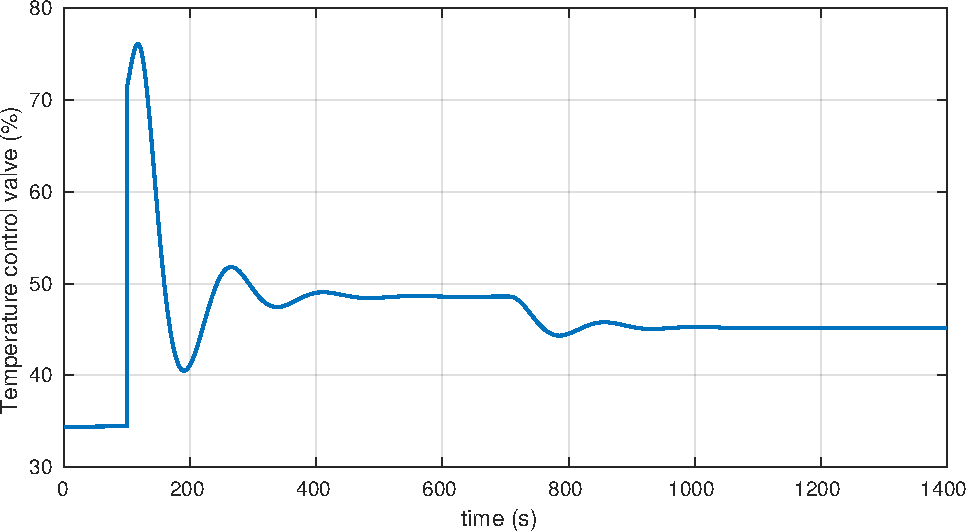
\includegraphics[width=\columnwidth]{Ch7CSTRControlledCV}
	\caption{Response of the controlled system using the nonlinear model for the CSTH.}
	\label{fig:Ch7CSTRControlledCV}
\end{figure}
%
Figure~\ref{fig:Ch7CSTRControlledCV}. When the setpoint change, the response of the controller is abrupt (more than double its original value), but then the value rapidly reach the new setpoint. The change produced by the disturbance has a milder response, and in less than \SI{200}{\second} reach again a new steady state.

The case presented here tried to show the steps to use the Pareto front as the methodology to find the controller tuning more appropriate to the task. The example is a simple plant, but very representative of the dynamics that can be found in an industry environment. Many of the plants can be modeled as a second order overdamped process, and therefore, the tool and the data used in this book are readily applied in many cases.

\subsection{PID control of the CSTH considering three integral cost functions}
\label{sec:PIDCSTH3Fun}
The MOOTuning software also is able to find the optimal parameters of a PID controllers considering three cost functions as presented in Section~\ref{sec:Tuning3PID}. Of course, it is not necessary to use this software since the data base with all the values is also part of the companion software, but the \matlab app has the advantage to be a simple interface between the user and the data.

As an example, the tuning tool is used to find the parameters of the controller that has the lowest $J_{do}$ value. This case is interesting because the anchor point where $J_{do}$ has the lowest value, neither the value of $J_r$ nor $J_{di}$ have their maximum value. On the other hand, when $J_{r}$ is set to be the lowest possible value, $J_{do}$ becomes the function that has an intermediate value but $J_{di}$ has its maximum value from the Pareto. Only for the anchor point where $J_{di}$ is minimum, both $J_r$ and $J_{do}$ get their maximum value. The responses for the three anchor points are depicted %
\begin{figure}[tb]
	\centering
	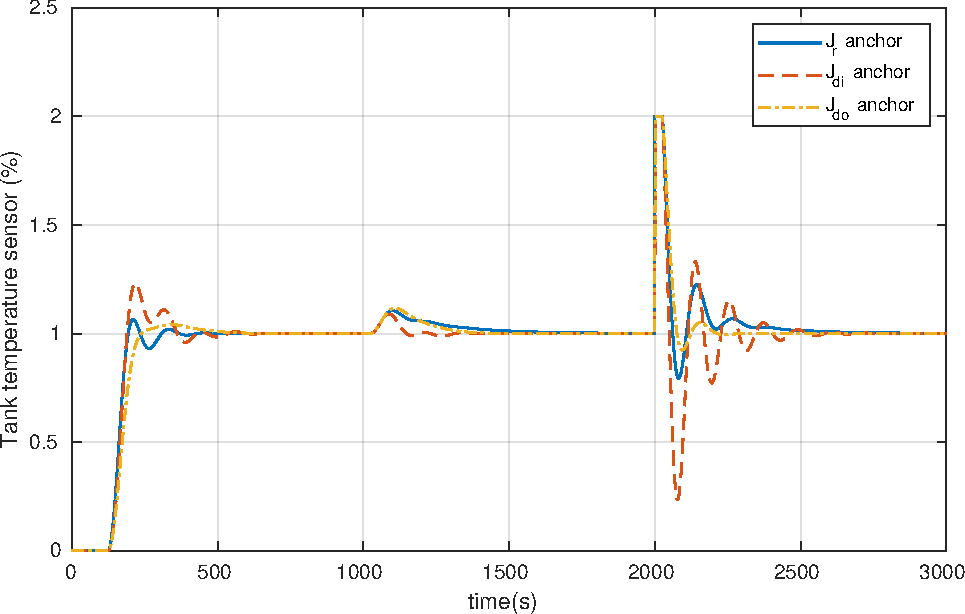
\includegraphics[width=\columnwidth]{Ch7CSTHControlled3Fun}
	\caption{Response of the CSTH process in the three anchor points of the pareto front for $M_s \leq 2.0$.}
	\label{fig:Ch7CSTHControlled3Fun}
\end{figure}
%
in Figure~\ref{fig:Ch7CSTHControlled3Fun} for the case where $M_s \leq 2.0$. As it can be seen, the response is quite different among the three anchor points. First a change in the reference value is performed at $t=\SI{100}{\second}$, an input step disturbance is present at $t=\SI{1000}{\second}$ and an output step disturbance is introduced in the system at $t=\SI{2000}{\second}$. The values of the cost functions are presented in %
%
\begin{table}
	\centering
	\caption{Cost functions for the three cost functions case scenario.}
	\begin{tabular}{cccc}
		\toprule
		 				& $J_r$ anchor point 					& $J_{di}$ anchor point				&	$J_{do}$ anchor point	\\
		 \midrule
		 $J_r$			&		$67.95$	(minimal)				&		$85.63$	($+26.02\%$)		&	$82.46$($+21.35\%$) \\
		 $J_{di}$		&		$22.46$ ($+218.13\%$)			&		$7.06$	(minimal)			&	$17.63$ ($+149.72\%$)	\\
		 $J_{do}$		&		$74.25$ ($+38.01\%$)			&		$102.43$ ($+90.39\%$)		&	$53.80$	(minimal)				\\
		 Parameters		& \begin{tabular}{c} $K_p = 8.19$ \\ $T_i = 185.18$\\ $T_d = 28.14$\\ $\beta = 0.99$		 \end{tabular} &
		 \begin{tabular}{c} $K_p = 11.29$ \\ $T_i = 58.8306$\\ $T_d = 29.48$\\ $\beta = 0.43$ \end{tabular} &
		 \begin{tabular}{c} $K_p = 6.18$ \\ $T_i = 108.76$\\ $T_d = 29.93$\\ $\beta = 0.82$ \end{tabular}\\
		 \bottomrule
	\end{tabular}
	\label{tab:2FunCostFunctionCSTH}
\end{table}
%
Table~\ref{tab:2FunCostFunctionCSTH}. The percentage increment is reported for each cost function in each case.

Using Figure~\ref{fig:Ch7CSTHControlled3Fun} and Table~\ref{tab:2FunCostFunctionCSTH} , it can be confirmed that the tuning with the best parameters for $J_{di}$ produces the worst responses for the other two functions. With these results one may be prone to select the tuning for the lowest value of $J_{di}$ as the final because it does not have the worst values of the other cost functions and it has much better response for the output disturbance case. Observe for example the response for the $J_{di}$ anchor point where the response for the output disturbance is bad (it has a $J_{do}$ increment of $+90.39\%$ with respect to its lowest value). In some sense, it could be seen as the best compromise between the cost functions. Only if the control engineer is heavily invested in minimize the $J_{di}$ cost function, it may select the $J_{di}$ anchor point as the final response, however, using the multiobjective framework presented here, he or she has to be fully aware that is selecting the worst response for the other functions.

Another reason to select the $J_{do}$ anchor point is related to the control effort. When the Total Variation computed as:
\begin{equation*}
TV = \sum_{i=0}^{N-1}\left(  u(i+1)-u(i)\right),
\end{equation*}
is compared between the three responses, it is found that $TV_{J_r} = 223.82$, $TV_{J_{di}} = 352.94$ and $TV_{J_{do}} = 152.81$ using a step size of $\SI{0.01}{\second}$. It is clear that the response given by the $J_{do}$ anchor point is a very good choice among all the possible values. The control signal is plotted %
%
\begin{figure}[tb]
	\centering
	\subfloat[Reference and input disturbance step changes.]{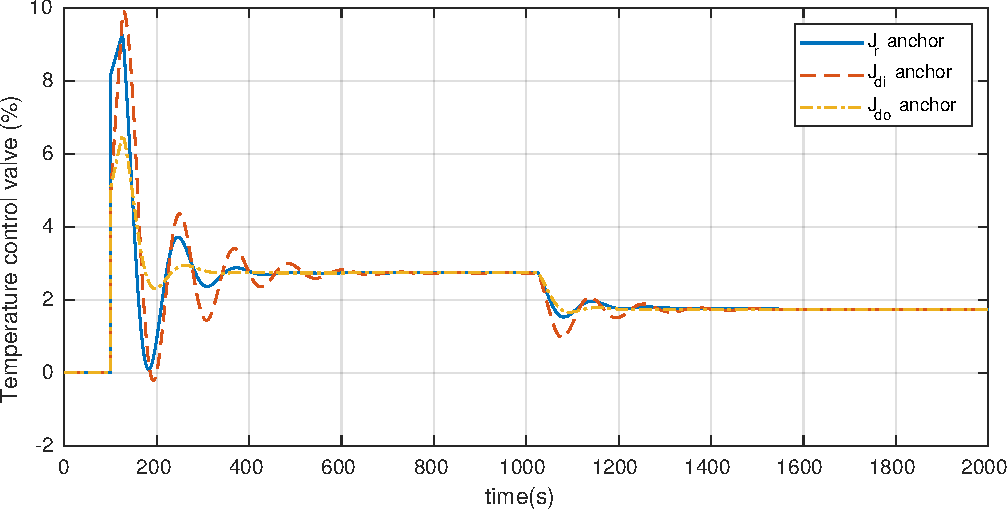
\includegraphics[width=\columnwidth]{Ch7CSTHControlledCV3Fun01} \label{fig:Ch7CSTHControlledCV3Fun01}}\\
	\subfloat[Output disturbance step change.]{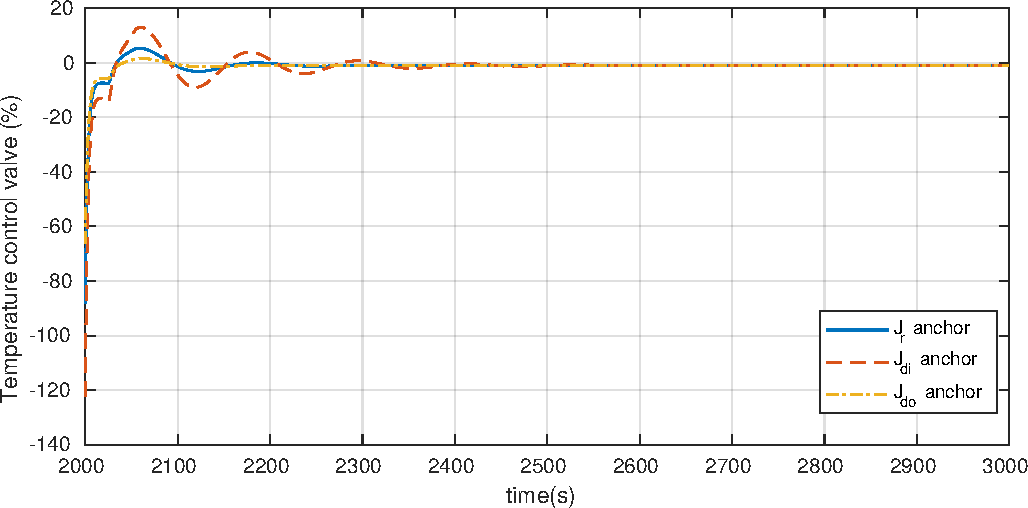
\includegraphics[width=\columnwidth]{Ch7CSTHControlledCV3Fun02} \label{fig:Ch7CSTHControlledCV3Fun02}}
	\caption{Control signal for the CSTH using three cost functions.}
	\label{fig:Ch7CSTHControlledCV3Fun}
\end{figure}
%
on Figure~\ref{fig:Ch7CSTHControlledCV3Fun}. Since the control signal has a larger magnitude for an output disturbance rejection, it was plotted in different axis.

As it can be seen from the response, effectively the response of the $J_{do}$ anchor point is smoother than the other two. Even if the control engineer is not looking for the best response to the output disturbance, the obtained tuning may be a good compromise between servo and regulation responses with a mild control signal.

In section~\ref{sec:PIDCSTH}, the system was controlled considering only two sources of disturbances. When adding another dimension to the problem, certainly the selection of the final controller may be more difficult because another degree of freedom is added. However, the insight that was gathered from rethinking the problem from this other point of view can be seen as beneficial, because the tuning found using the 3 dimensional Pareto could be a better solution (from a physical point of view) that may not be part of the front with only two functions.
%
% -----------------------------------------------------------------------------------------------------------
%
\section{Continuous Stirred Tank Reactor}
\label{sec:CSTRVandeVusse}
%
\subsection{Description of the process}
\label{sec:DescriptionCSTR}

The \gls{cstr} with the Van de Vusse reaction \citep{VandeVusse1964} is a common benchmark plant for testing control algorithms given its different dynamics depending on the operating point and is depicted in %
\begin{figure}[tb]
	\centering
	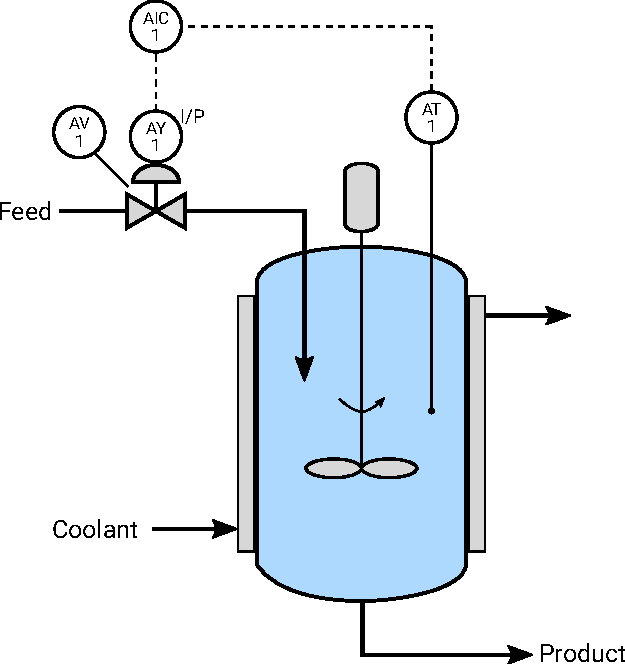
\includegraphics[scale=0.6]{Ch7VandeVusse}
	\caption{\gls{cstr} process using the Van de Vusse reaction model.}
	\label{fig:Ch7VandeVusse}
\end{figure}
%
Figure~\ref{fig:Ch7VandeVusse}. For this particular case, the isothermal process is considered and both the concentration sensor as the valve actuator will be modeled as well. The objective is to control the feed flow to obtain the desired concentration of a product.

The Van de Vusse reaction models a process where desired product B is obtained from A, but at the same time, both A and B are degraded to D and C respectively. The chemical equation that represent this reaction is given by:
%
\begin{align*}
A &\overset{k_1}{\longrightarrow} B \overset{k_2}{\longrightarrow}C,\\
2 A &\overset{k_3}{\longrightarrow} D,
\end{align*}
%
where $k_i$ are the rate constants of the formation rates of A and product B as given by \citep{VandeVusse1964}:
\begin{equation}
\begin{split}
r_A &= -k_1 A - k_3 A^2,\\
r_B &= k_1 A - k_2 B.
\end{split}
\label{eq:RateVandeVusse}
\end{equation}

When performing a mass balance, the model becomes \citep{Arrieta2010}:
%
\begin{equation}
\begin{split}
\frac{dC_A(t)}{dt} & = \frac{F_r(t)}{V} \left(C_{Ai}-C_A(t)\right) - k_1 C_A(t) - k_3 C^2_A(t)\\
\frac{dC_B(t)}{dt} & = -\frac{F_r(t)}{V} C_B(t)+ k_1 C_A(t) - k_2 C_B(t)
\end{split}
\label{eq:CSTRMVE}
\end{equation}
%
where $C_A$ and $C_B$ represents the reactants concentrations  in \si{\mole\per\liter}, $C_{Ai}$ is the concentration of A in the feed flow in \si{\mole\per\liter}, $F_r$ is the input flow in \si{\liter\per\minute}, and $V$ is the volume of the \gls{cstr} in \si{\liter}. The nominal values of the parameters are presented in %
%
\begin{table}[tb]
	\centering
	\caption{Parameters values for the \gls{cstr} model.}
	\begin{tabular}{cc}
		\toprule
		$k_1 = \SI{0.833}{\per\minute}$ & $k_2 = \SI{1.667}{\per\minute}$ \\
		$k_3 = \SI{0.167}{\per\minute}$ & $C_{Ai} = \SI{10}{\mole\per\liter}$\\
		$V = \SI{700}{\liter}$\\
		\bottomrule
	\end{tabular}
	\label{tab:ParamCSTR}
\end{table}
%

The range of the sensor for the product is supposed to be in the range 0 to \SI{1.5714}{\mole\per\liter} and the maximum flow that is allowed by the valve is given by \SI{634.1719}{\liter\per\minute}. Given these values, the model for the sensor-transmitter is given by:
\begin{equation}
	y(t) = \left(\frac{100}{1.5714}\right) C_B(t),
	\label{eq:Sensor}
\end{equation}
%
while the transmitter is modeled as:
\begin{equation}
F_r(t) = \left(\frac{634.1719}{100}\right) u(t),
\label{eq:Transmiter}
\end{equation}
%
where $u(t)$ and $y(t)$ are the normalized input and output signal, respectively. The operation point of the plant is given by $u_0 = 60\%$ and $y_0 = 70\%$ which represents concentration of $C_{A0} = \SI{2.9175}{\mole\per\liter}$ and $C_{B0} = \SI{1.10}{\mole\per\liter}$ with the input concentration given by $C_{Ai0} = \SI{10}{\mole\per\liter}$.

These parameters give the system a wide range of operation. In %
\begin{figure}
	\centering
	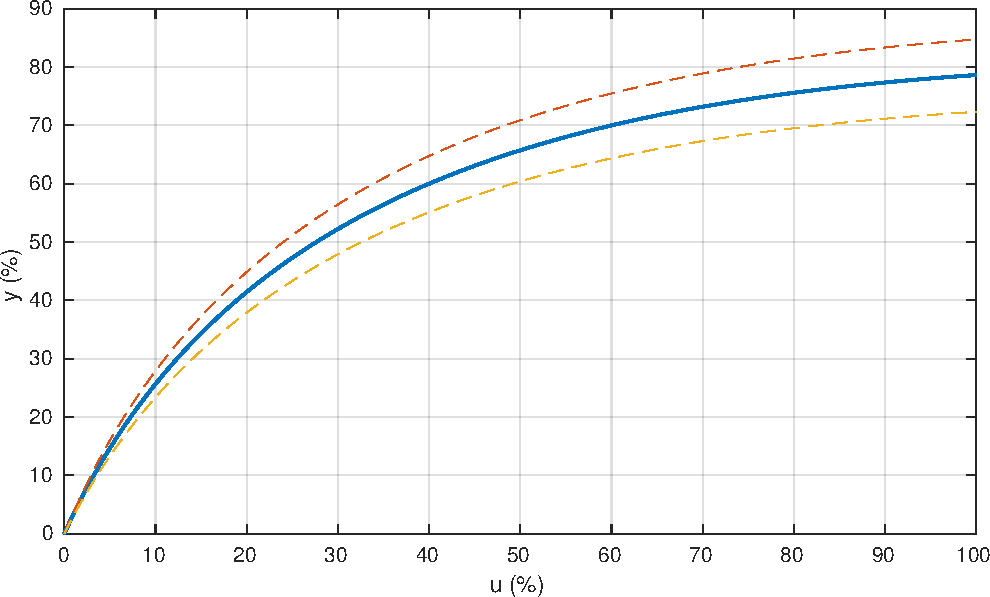
\includegraphics[width=\columnwidth]{Ch7VandeVusseOP}
	\caption{Operation points of the \gls{cstr} process.}
	\label{fig:Ch7VandeVusseOP}
\end{figure}
Figure~\ref{fig:Ch7VandeVusseOP} it can be seen that with the value of $C_{Ai0}$ given and the input at $60\%$, the output yield $70\%$. In the figure the dashed lines represents the variation due to $\pm 10\%$ variation of $C_{Ai}$. It can be seen that, with a $100 \%$ value for $u$ and a variation of $10\%$ of $C_{Ai}$, the output is less than $100\%$ of the capacity of the sensor.

The concentration of $C_a$ and $C_b$ are both plotted in %
\begin{figure}
	\centering
	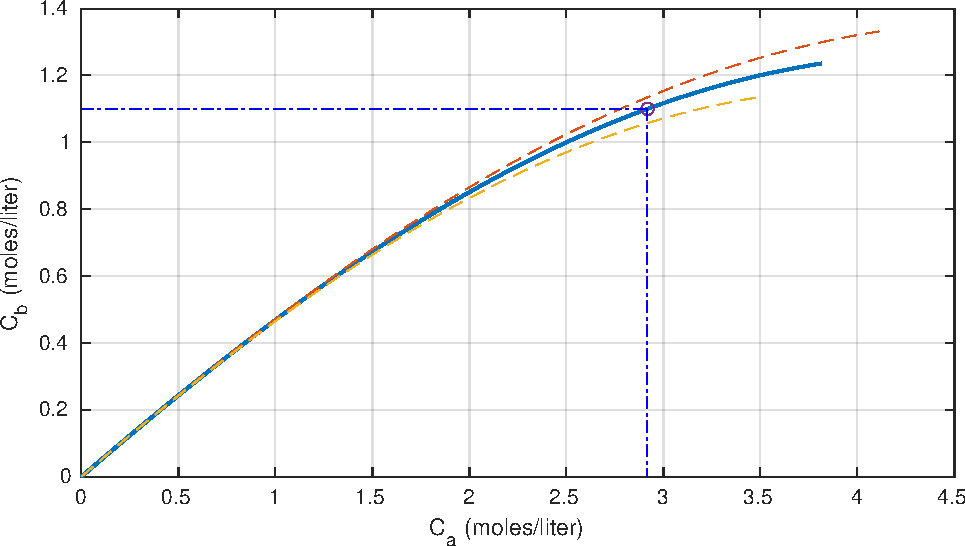
\includegraphics[width=\linewidth]{Ch7VandeVusseOPStates}
	\caption{Concentration of the reactants for all possible operating points.}
	\label{fig:Ch7VandeVusseOPStates}
\end{figure}
%
Figure~\ref{fig:Ch7VandeVusseOPStates}. The $C_a$ concentration is on the horizontal axis is while the $C_b$ concentration is on the vertical axis. The selected operation point is represented with a circle in the curve and also the curves with the variation on the value of $C_{Ai}$ are also presented. As it can be seen, in the operation point selected, the curves start to diverge, which means that the model has a larger dependency on the variation of the input concentration. This has to be taken into account when designing the feedback controller.

When considering the transient response to a change in the input flow $u$, the response is as given in %
\begin{figure}
	\centering
	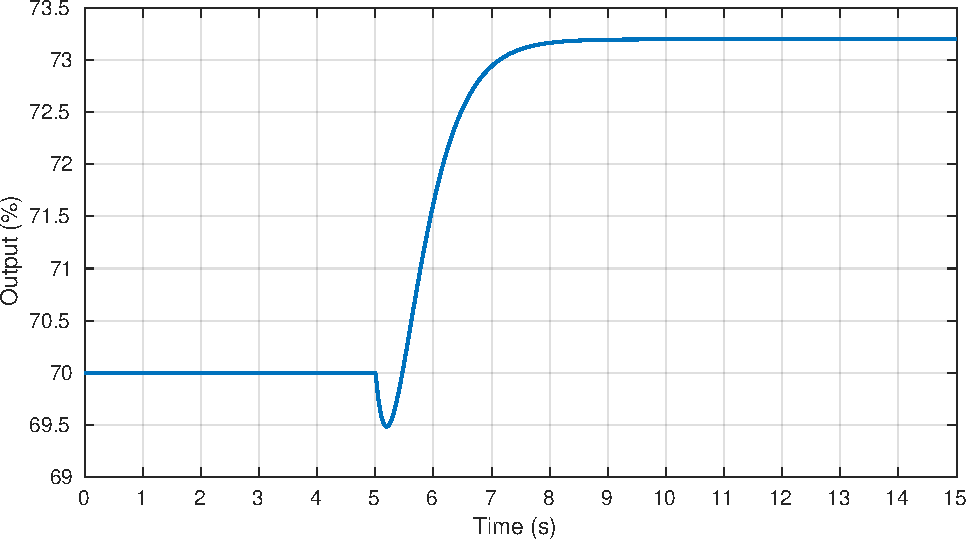
\includegraphics[width=\linewidth]{Ch7VandeVusseStep}
	\caption{Open loop response to a step change in the input signal of the \gls{cstr}.}
	\label{fig:Ch7VandeVusseStep}
\end{figure}
%
Figure~\ref{fig:Ch7VandeVusseStep}. It is interesting to note that the the system has an inverse response. This characteristic limits the possible performance of the controlled loop, making unfeasible to increase the gain of the controller to achieve a faster response without instability. This is also another point that has to be considered when designing the controller.

This model was implemented as an S-Function in \matlab/\simulink and can be found in the companion software. In %
\begin{figure}[tb]
	\centering
	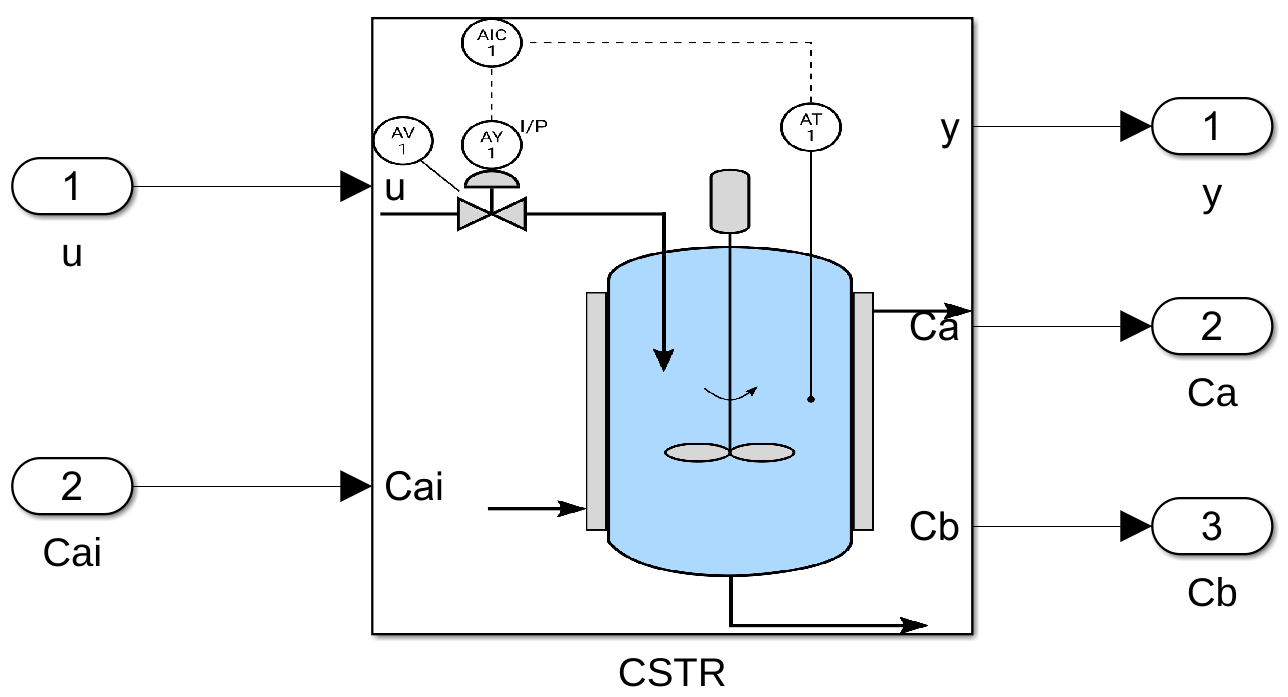
\includegraphics[width=\linewidth]{Ch7CSTRSimulinkSystem}
	\caption{CSTR implemented as an S-function in \simulink.}
	\label{fig:Ch7CSTRSimulinkSystem}
\end{figure}
%
Figure~\ref{fig:Ch7CSTRSimulinkSystem}, the basic block with the model is presented. It has $u$ and $C_{ai}$ as inputs and $y$, $C_a$ and $C_b$ as outputs. With the intention to facilitate the characterization of the model, a mask was designed to enter the parameters and the initial value of the states. This mask can be found in %
\begin{figure}[tb]
	\centering
	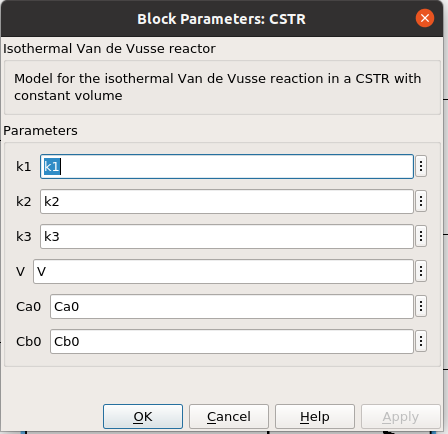
\includegraphics[width=0.5\linewidth]{Ch7VandeVusseParamWindow}
	\caption{\simulink mask to enter parameters and initial values for the \gls{cstr} system.}
	\label{fig:Ch7VandeVusseParamWindow}
\end{figure}  
Figure~\ref{fig:Ch7VandeVusseParamWindow}. All the values of the parameters can be set on the \matlab workspace and use directly on the mask. This is and advantage in case the user desires to use another set of parameters or compare the response of the system with different values.

The objective of this example is to control the reactor using the multiobjective approach. In order to use the framework and the \matlab app, it is necessary to find a suitable linear second order model. Next, the procedure to find this model is presented.

\subsection{Linearization}
\label{sec:CSTRLin}
In order to use the MOOTuning software, it is necessary to have a linear model of the process. In this case, the linearization is done by taking the first order approximation of the model in \eqref{eq:CSTRMVE} near the operation point.

When defining the incremental variables $\mathbf{\delta x}$, $\mathbf{\delta u}$ and $\delta y$ as:
\begin{align*}
\mathbf{\delta x} &= \left[ \begin{array}{c} C_A - C_{A0} \\ C_B - C_{B0} \end{array} \right], \\
\mathbf{\delta u} &= \left[ \begin{array}{c} u-u_0 \\ C_{Ai} - C_{Ai0} \end{array} \right], \\
\delta y &= y - y_0 .
\end{align*}

The process dynamics can be approximated by the first order model given by:
%
\begin{align}
\dot{\mathbf{\delta x}} &=  \mathbf{A}\mathbf{\delta x} + \mathbf{B} \mathbf{\delta u}, \\
%
\delta y &=  \mathbf{C} \mathbf{\delta x},
\end{align}
%
where,
\begin{align*}
	\mathbf{A} &= \left[ \begin{array}{cc} \frac{6.341719 u_0}{V} - k1 - 2 k_3 C_{A0} & 0 \\ k1 & \frac{-6.341719 u_0}{V} - k_2 \end{array}\right],\\
	\mathbf{B} &= \left[ \begin{array}{cc} \frac{6.341719 (C_{Ai0}-C_{A0})}{V} & \frac{6.341719 u_0}{V} \\ \frac{-6.341719 C_{B0}}{V} & 0 \end{array} \right], \\
	\mathbf{C} &= \left[ \begin{array}{cc} 0 & \frac{100}{1.5714} \end{array} \right].
\end{align*}

Using the parameters of Table~\ref{tab:ParamCSTR} and the operation point values, the resulting transfer function between input $u$ and output $y$ is found to be:
\begin{equation}
	F(s) = \frac{-0.6342 s + 1.913}{s^2 + 4.56 s + 5.193}
	\label{eq:TFCSTR}
\end{equation}

It has to be clear that this transfer function is only an approximation of the model, and therefore it is valid only around the operating point. When a step change of $5\%$ is entered in the system, the response of the nonlinear model and the response of the transfer function start to differ as presented in %
%
\begin{figure}[tb]
	\centering
	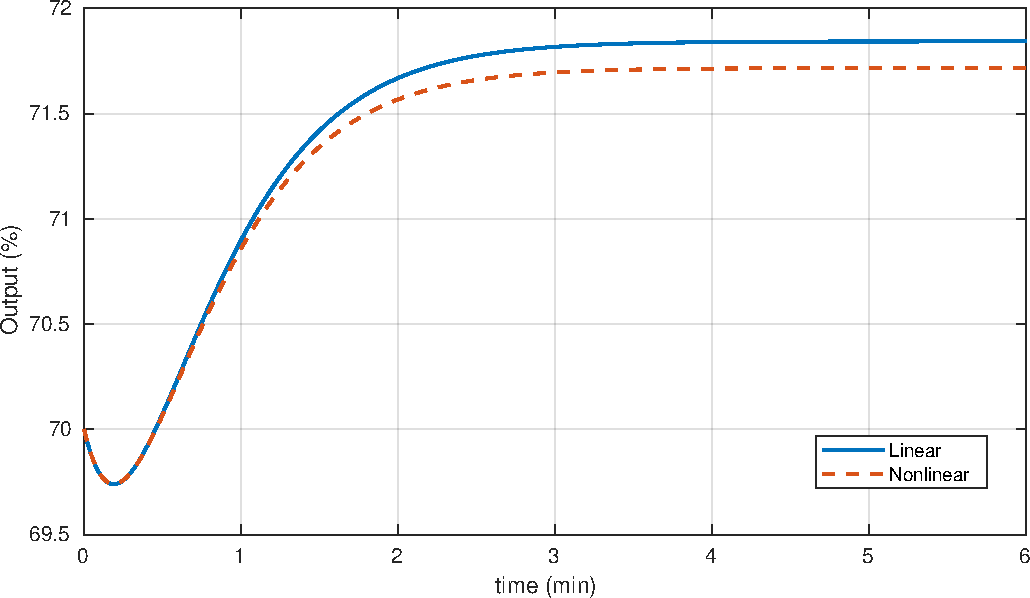
\includegraphics[width=\linewidth]{Ch7CSTRLinear}
	\caption{Comparison of the nonlinear and linear model for the \gls{cstr} for a 5\% change in the input.}
	\label{fig:Ch7CSTRLinear}
\end{figure}
%
Figure~\ref{fig:Ch7CSTRLinear}. As it can be seen, the linear model represents the transient response well, however it fails to predict the steady state. Of course, the smaller the change in the input, the better is the the approximation for both the transient and the steady state response.

However, the model that is expected in the \matlab app does not contemplate a non-minimum phase zero in the model. Using the model reduction rules of \citet{Skogestad2003}, the \gls{soptd} model ends as:
\begin{equation}
	F_{aprox} = \frac{0.368 e^{-0.331}}{0.193 s^2 + 0.878 s +1}.
	\label{eq:Faprox}
\end{equation}
which corresponds to approximate the non-minimum phase zero by a time delay. The gain is given by $K=0.3684$, the time constant is given by $\tau= \SI{0.4256}{\minute}$, the time delay is $L= \SI{0.3315}{\minute}$ and $a = 0.9408$. This new transfer function gives the response presented in %
\begin{figure}[tb]
	\centering
	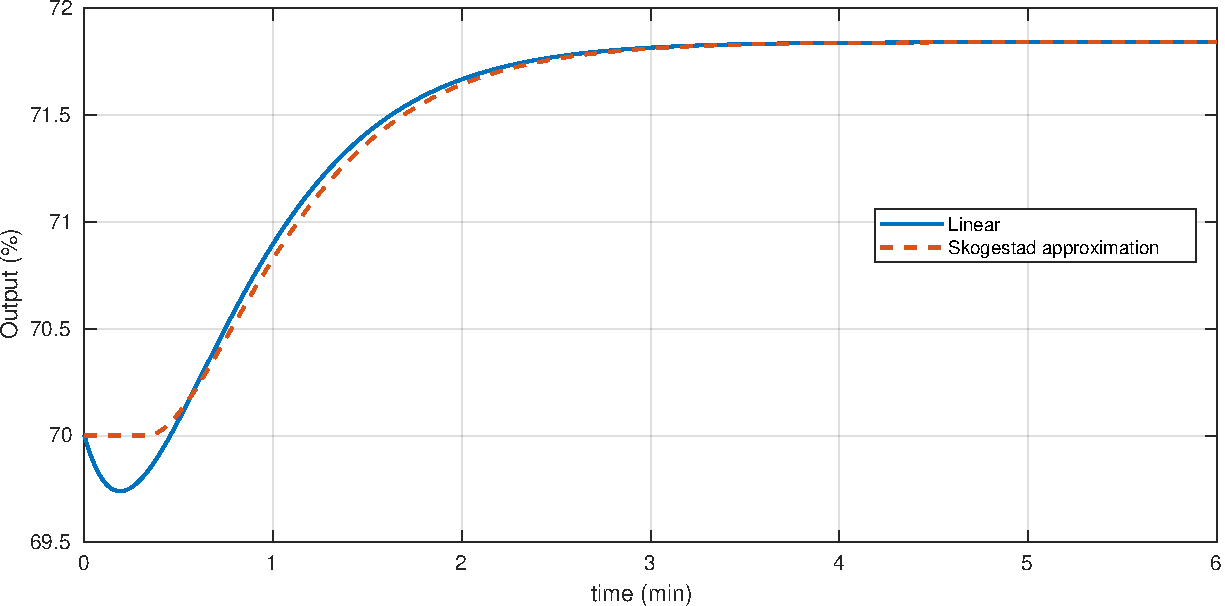
\includegraphics[width=\linewidth]{Ch7CSTRLinearSkogestad}
	\caption{Approximation of the non-minimum phase zero with a time delay for the linear model of the \gls{cstr}.}
	\label{fig:Ch7CSTRLinearSkogestad}
\end{figure}
%
Figure~\ref{fig:Ch7CSTRLinearSkogestad}. Of course, the dynamic model is quite different from the original nonlinear model, both in the transient and steady states. Since the controller is going to be designed with the linearized time-delayed transfer function, it is necessary to consider some restriction on the performance in order to give certain robustness to the design.

\subsection{Controller design}
For this particular example, the design of the controller parameters will contemplate three different robustness cases: without any restriction to the value of \gls{ms}, $M_s = 2.0$ and $M_s = 1.8$. The MOOTuning app is able to introduce the robustness as a restriction in the design. However, it is limited to certain values of $M_s$ which are considered to be reasonable for an industrial control applications.

In this particular example, only $J_{r}$ and $J_{di}$ are going to be considered. The design is based on the model in \eqref{eq:Faprox} and will be tested on the nonlinear model as well. Several points of the Pareto are going to be tested: the two anchor points (C1 for best regulator and C2 for best servo), the best regulator possible with a 20\% degradation on $J_r$ (C3) and the best servo possible with a 20\% degradation on $J_{di}$ (C4).
%
\begin{table}[tb]
	\caption{Different tunings for the \gls{cstr} obtained with MOOTuning.}
	\centering
	\begin{tabular}{m{1cm}m{1cm}m{1cm}m{1cm}m{1cm}m{1cm}m{1cm}}
		\toprule
		Design & $K_p$ & $T_i$ & $T_d$ & $\beta$ & $J_{di}$ & $J_r$ \\
		\midrule
		\multicolumn{7}{c}{$M_s \geq 2.0$} \\
		\midrule
		C1 & 6.00 & 0.61 & 0.29 & 0.49 & 0.13 & 0.98\\
		C2 & 4.54 & 1.24 & 0.26 & 0.99 & 0.27 & 0.80\\
		C3 & 5.54 & 0.85 & 0.26 & 0.66 & 0.14 & 0.85\\
		C4 & 5.33 & 0.91 & 0.26 & 0.73 & 0.17 & 0.84\\
		\midrule
		\multicolumn{7}{c}{$M_s = 2.0$} \\
		\midrule
		C1 & 4.43 & 0.76 & 0.21 & 0.66 & 0.17 & 0.92\\
		C2 & 4.29 & 1.19 & 0.25 & 0.99 & 0.28 & 0.80\\
		C3 & 4.44 & 0.86 & 0.22 & 0.73 & 0.19 & 0.86\\
		C4 & 4.40 & 1.00 & 0.24 & 0.87 & 0.23 & 0.83\\
		\midrule
		\multicolumn{7}{c}{$M_s = 1.8$} \\
		\midrule
		C1 & 3.88 & 0.72 & 0.22 & 0.72 & 0.20 & 0.98\\
		C2 & 3.86 & 1.13 & 0.24 & 0.99 & 0.29 & 0.82\\
		C3 & 3.91 & 0.85 & 0.21 & 0.75 & 0.22 & 0.89\\
		C4 & 3.92 & 0.96 & 0.22 & 0.87 & 0.24 & 0.85\\
		\bottomrule
	\end{tabular}
	\label{tab:CSTRDesigns}
\end{table}

All the tuning values for the cases studied are presented in Table~\ref{tab:CSTRDesigns}. In general, it can be seen that the proportional gain is heavily dependent of the robustness value (more robustness implies lower values of $K_p$). On the other hand it seems that the value of $T_i$ is more dependent of the degradation of $J_{di}$ while the variation of $T_d$ is small across all cases. The value of $\beta$ seems like a combination of the degradation of $J_{di}$ and the value of the robustness.

To compare the responses, it is useful to plot the step response of C1 controllers across all robustness values as presented in %
\begin{figure}[tb]
	\centering
	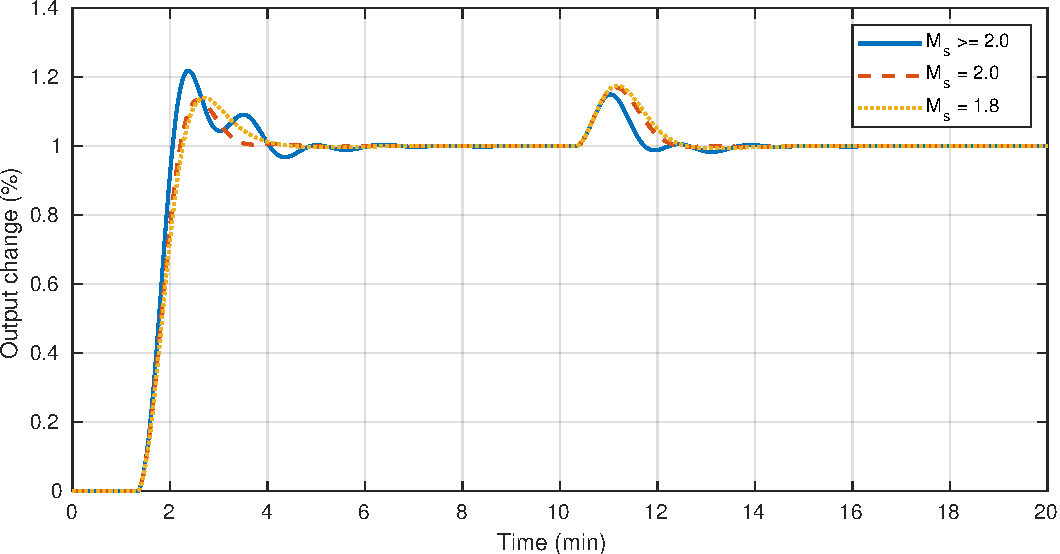
\includegraphics[width=\linewidth]{Ch7CSTRControlC1}
	\caption{Response for C1 controllers for all $M_s$ values.}
	\label{fig:Ch7CSTRControlC1}
\end{figure}
%
Figure~\ref{fig:Ch7CSTRControlC1} and for C2 controllers as in %
\begin{figure}[tb]
	\centering
	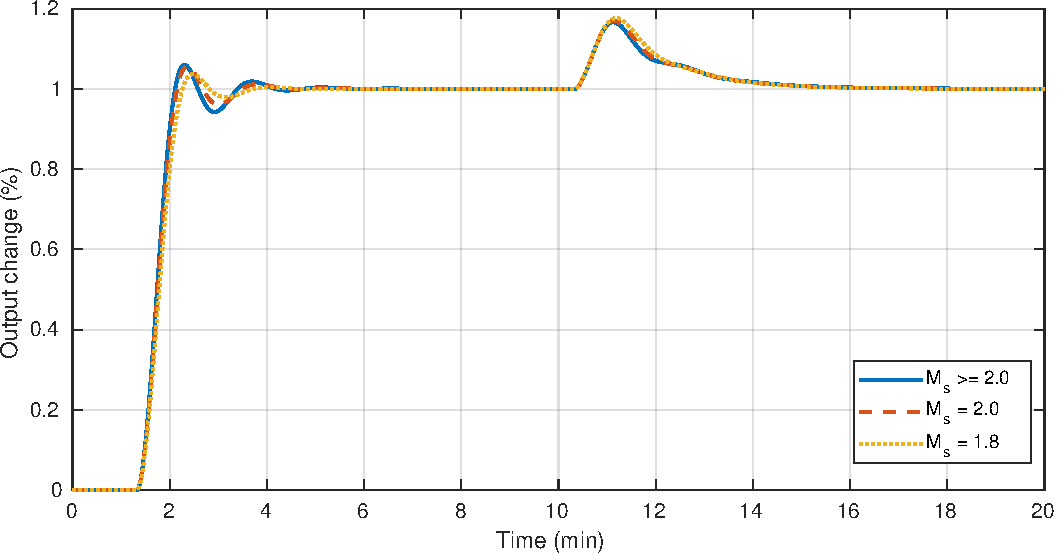
\includegraphics[width=\linewidth]{Ch7CSTRControlC2}
	\caption{Response for C2 controllers for all $M_s$ values.}
	\label{fig:Ch7CSTRControlC2}
\end{figure}
%
Figure~\ref{fig:Ch7CSTRControlC2}. It is interesting to note that C1 controllers presents more variability in the response with respect to the controllers of the C2 family. In both figures it is clear that there is a compromise between the servo and the regulator responses, but this compromise becomes less important when the robustness is considered. Consider Figure~\ref{fig:Ch7CSTRControlC1}, the response for $M_s \geq 2.0$ does not take into account any constraint on the robustness and as it can be seen this response is very different than the cases where $M_s = 2.0$ and $M_s = 1.8$ are forced. It has to be noticed that adding the robustness constraint greatly limits the possible values of the controllers.

On the other hand, it was found that for the C2 controllers family the responses are very similar among all robustness, as can be seen in Figure~\ref{fig:Ch7CSTRControlC2}. The reason for this is the parameter $\beta$. This parameter does not affect the robustness value of the controlled system nor the regulator response. Therefore, the optimization tend to find a low value for $K_p$, which gives better robustness, but then compensates with a high value of $\beta$.

The control signals for the controllers are presented in Figures~\ref{fig:Ch7CSTRControlC1U} and \ref{fig:Ch7CSTRControlC2U}. %
\begin{figure}[tb]
	\centering
	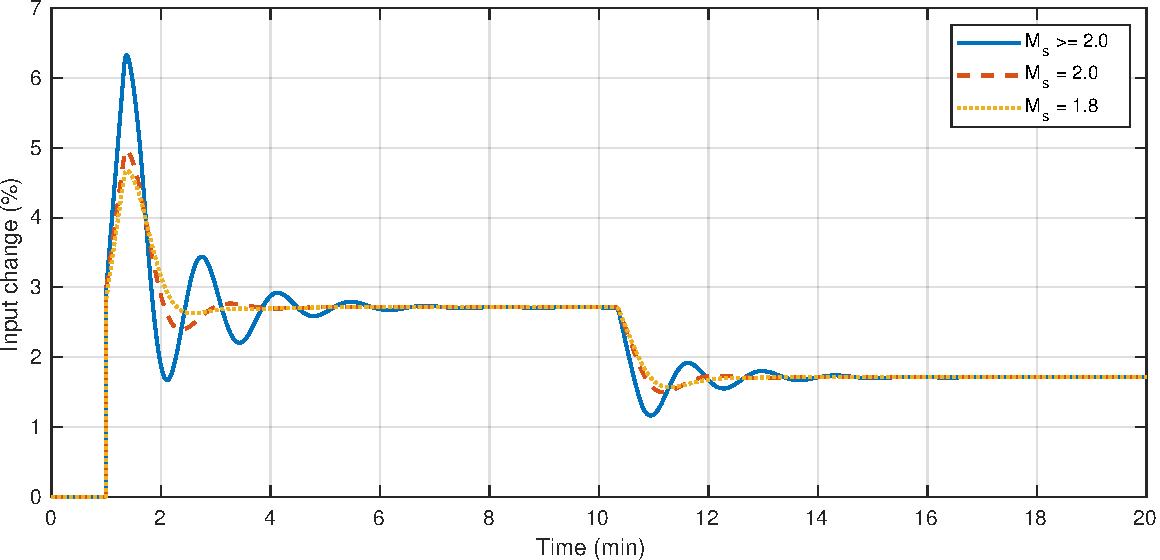
\includegraphics[width=\linewidth]{Ch7CSTRControlC1U}
	\caption{Control signal for C1 controllers for all $M_s$ values.}
	\label{fig:Ch7CSTRControlC1U}
\end{figure}
%
\begin{figure}[tb]
	\centering
	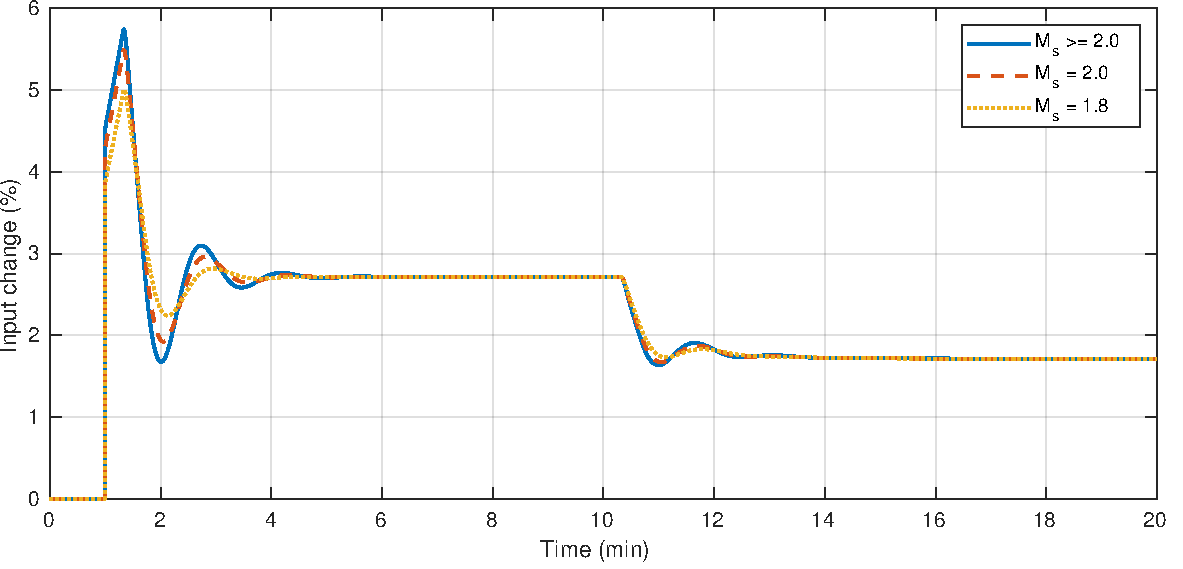
\includegraphics[width=\linewidth]{Ch7CSTRControlC2U}
	\caption{Control signal for C2 controllers for all $M_s$ values.}
	\label{fig:Ch7CSTRControlC2U}
\end{figure}
%
For the case of C1 controllers, the control signal varies significantly according to the robustness value. The case without any constraint has a larger peak and more oscillatory response than any of the other controllers. It is interesting, however, to note that the control signal for the C2 controllers are very similar and again, this is due to the presence of the $\beta$ parameter. The fact that an unconstrained controller may be applied to the controlled system has to be taken with caution, because in this design, the model used for the controller tuning is known to be different that the system. Therefore, applying an aggressive control signal may lead to unwanted oscillatory behavior and even instability.

Now, the responses of the different controllers families can be compared for the same given robustness, for example $M_s = 2.0$ as in %
\begin{figure}[tb]
	\centering
	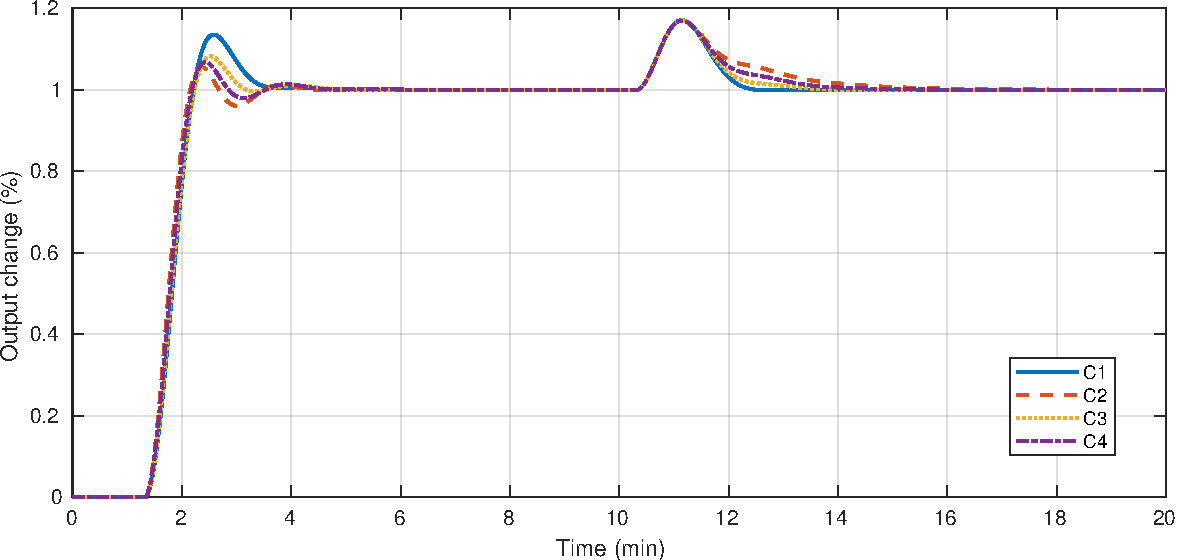
\includegraphics[width=\linewidth]{Ch7CSTRControlMs2}
	\caption{Response for all controller families with $M_s = 2.0$.}
	\label{fig:Ch7CSTRControlMs2}
\end{figure}
%
Figure~\ref{fig:Ch7CSTRControlMs2}. For all this controllers, the robustness is near $M_s = 2.0$, but the performance is varied from $J_r$ and $J_{di}$. Here, the compromise between both responses is clearer since the best servo is at the same time the worst regulator and the best regulator is the worst servo.
%
\begin{figure}[tb]
	\centering
	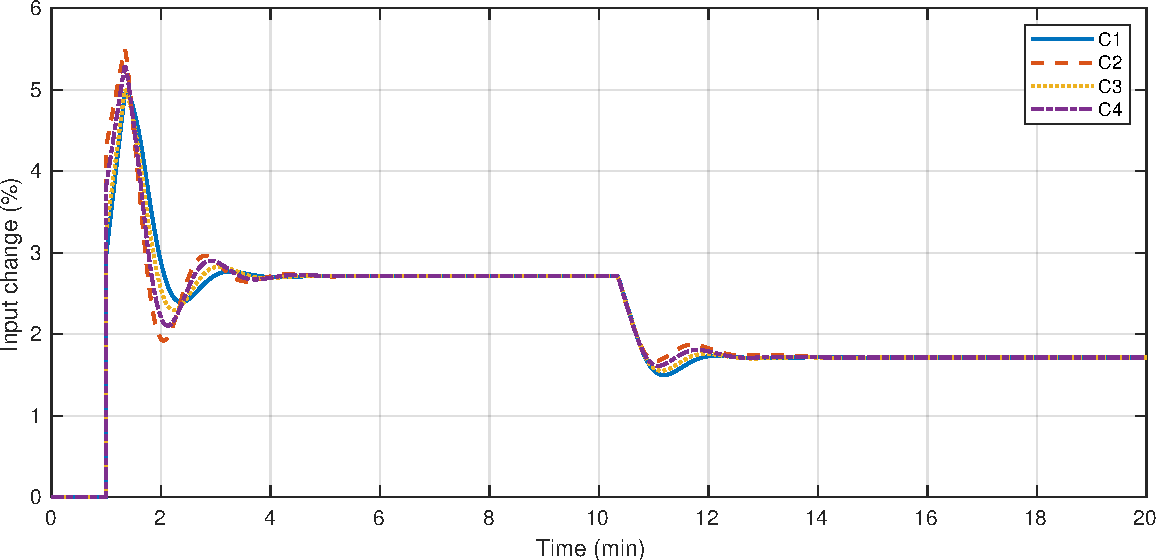
\includegraphics[width=\linewidth]{Ch7CSTRControlMs2U}
	\caption{Control signal for all controller families with $M_s = 2.0$.}
	\label{fig:Ch7CSTRControlMs2U}
\end{figure}
%

However, given that all controllers are constraint to fulfill $M_s = 2.0$, the difference between them are not very notorious. It can be seen on Figure~\ref{fig:Ch7CSTRControlMs2U} that the peaks and oscillatory behavior of all controllers are practically the same. When the robustness became too thing (for example values below 1.4) the controllers for servo and regulator practically become the same and the degree of freedom to select the dynamic behavior is practically non-existent.

\subsection{Validation of the controller designs}
\label{sec:ValidationCSTR}
%
The designed controllers were tested using the nonlinear model of the \gls{cstr}. It is important to note that the controllers were tuned for a plant model that is different than the ``real'' plant. In this particular case, several approximations where made which were necessary in order to use the framework presented in the other chapters. Because of this, it is important to look for a solution that takes into account this possible sources of instability.
%
\begin{table}[tb]
	\centering
	\caption{IAE values for the controllers applied to the nonlinear model as servo controllers}
	\begin{tabular}{p{1.5cm}>{\centering}p{1cm}>{\centering}p{1cm}>{\centering}p{1cm}>{\centering\arraybackslash}p{1cm}}
		\toprule
		\multirow{2}{*}{Robustness}	& \multicolumn{4}{c}{Controller}\\
		\cmidrule{2-5}
									& C1 & C2 & C3 & C4 \\
		\midrule
		$M_s = 1.8$ & 0.94 & 0.83 & 0.87 & 0.84\\
		$M_s = 2.0$ & 0.86 & 0.79 & 0.83 & 0.81\\
		$M_s \geq 2.0$ & 11.20 & 0.78 & 1.02 & 0.83\\
		\bottomrule
	\end{tabular}
	\label{tab:CSTRIAEServo}
\end{table}
%
\begin{table}[tb]
	\centering
	\caption{TV values for the controllers applied to the nonlinear model as servo controllers}
	\begin{tabular}{p{1.5cm}>{\centering}p{1cm}>{\centering}p{1cm}>{\centering}p{1cm}>{\centering\arraybackslash}p{1cm}}
		\toprule
		\multirow{2}{*}{Robustness}	& \multicolumn{4}{c}{Controller}\\
		\cmidrule{2-5}
		& C1 & C2 & C3 & C4 \\
		\midrule
		$M_s = 1.8$ & 9.40 & 13.20 & 9.14 & 11.10\\
		$M_s = 2.0$ & 11.34 & 20.01 & 12.75 & 16.37\\
		$M_s \geq 2.0$ & 1936.10 & 29.10 & 128.30 & 73.20\\
		\bottomrule
	\end{tabular}
	\label{tab:CSTRTVServo}
\end{table}
%
\begin{figure}
	\centering
	\subfloat[$M_s = 2.0$]{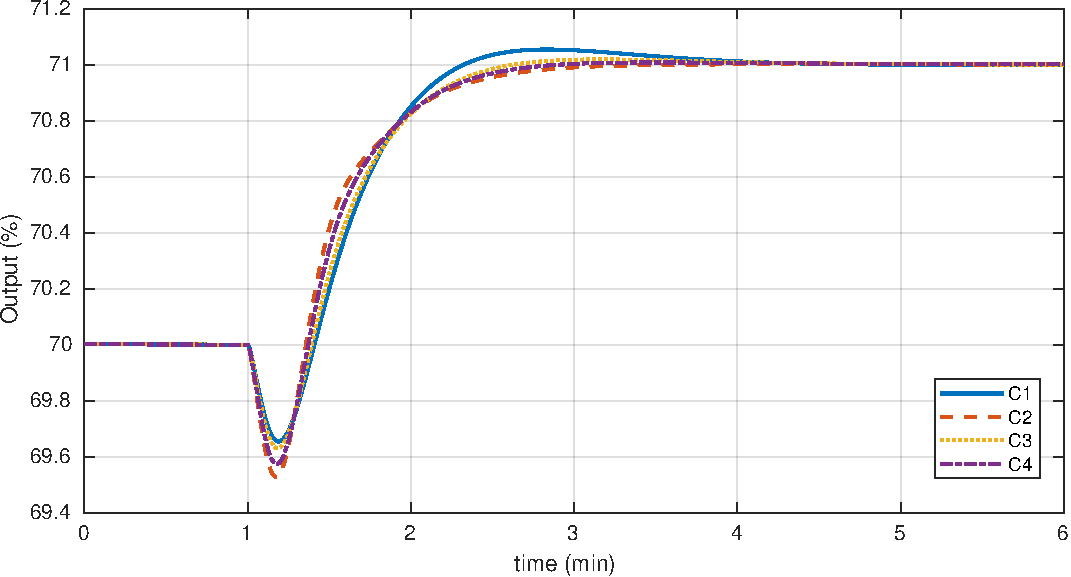
\includegraphics[width=0.8\linewidth]{CH7CSTRControlServoMs2Y} \label{fig:CH7CSTRControlServoMs2Y}}\\
	\subfloat[$M_s = 1.8$]{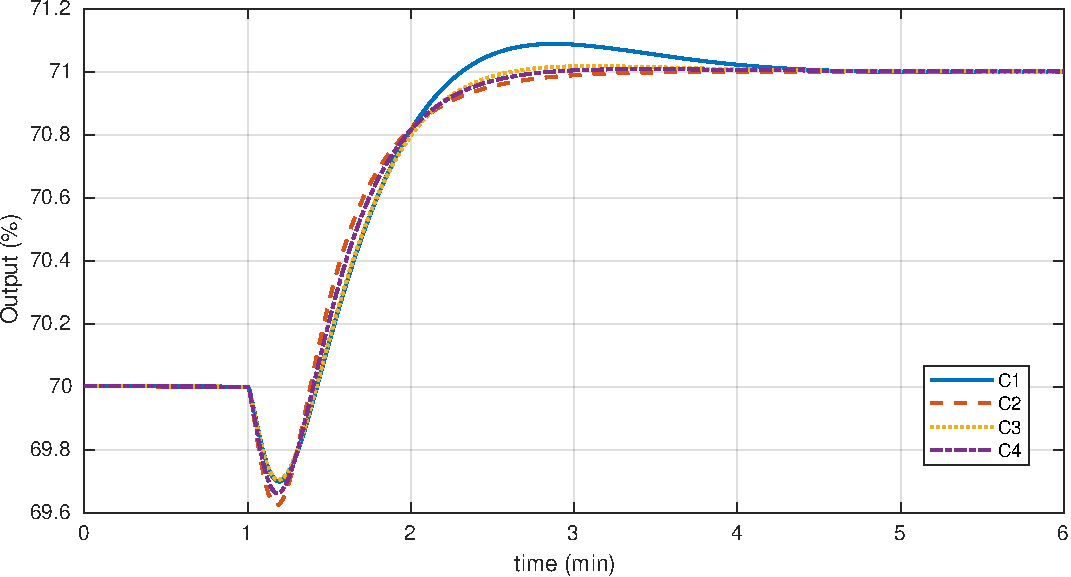
\includegraphics[width=0.8\linewidth]{CH7CSTRControlServoMs18Y} \label{fig:CH7CSTRControlServoMs18Y}}\\
	\subfloat[$M_s \geq 2$]{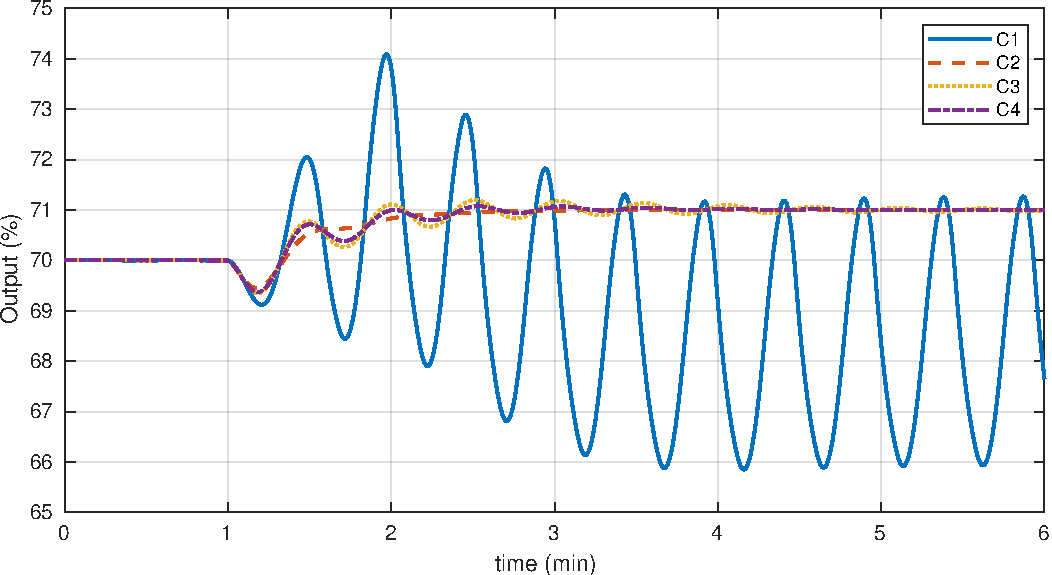
\includegraphics[width=0.8\linewidth]{CH7CSTRControlServoMs10Y} \label{fig:CH7CSTRControlServoMs10Y}}
	\caption{Response of the controlled system with the nonlinear model for several robustness levels serving as servo.}
	\label{fig:CH7CSTRControlServoY}
\end{figure}
%
%
\begin{figure}
	\centering
	\subfloat[$M_s = 2.0$]{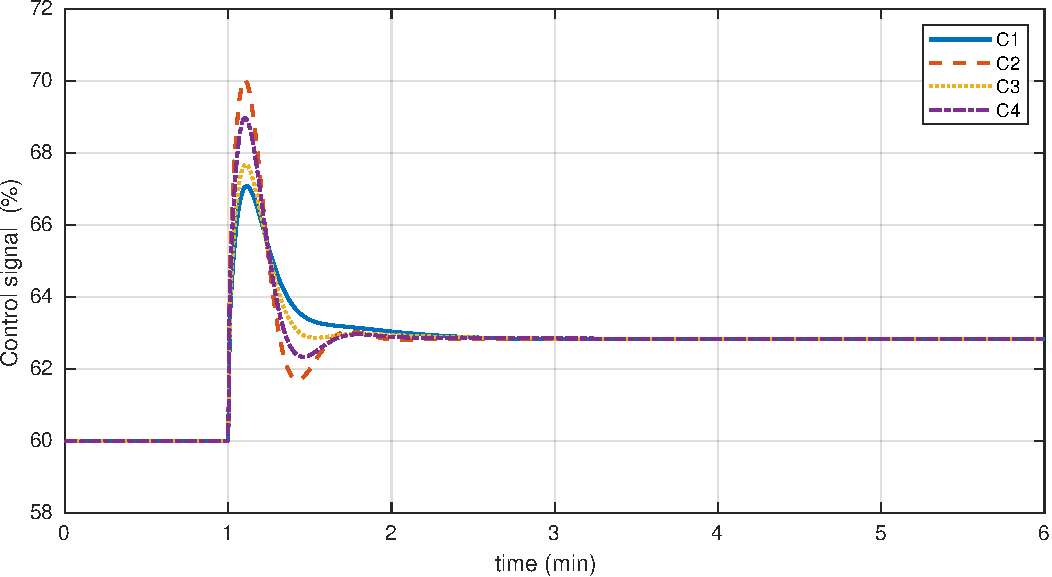
\includegraphics[width=0.8\linewidth]{CH7CSTRControlServoMs2U} \label{fig:CH7CSTRControlServoMs2U}}\\
	\subfloat[$M_s = 1.8$]{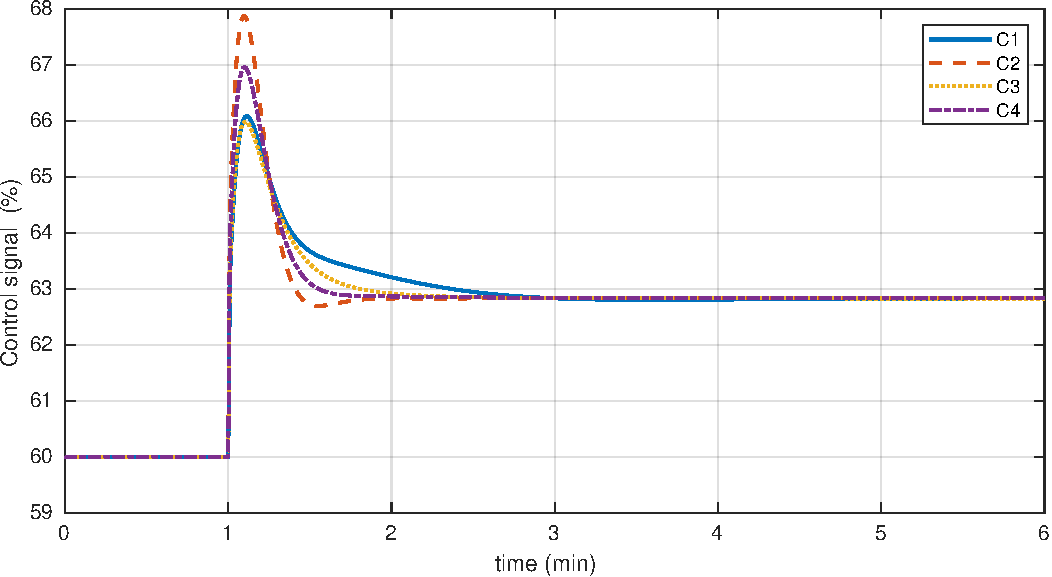
\includegraphics[width=0.8\linewidth]{CH7CSTRControlServoMs18U} \label{fig:CH7CSTRControlServoMs18U}}\\
	\subfloat[$M_s \geq 2$]{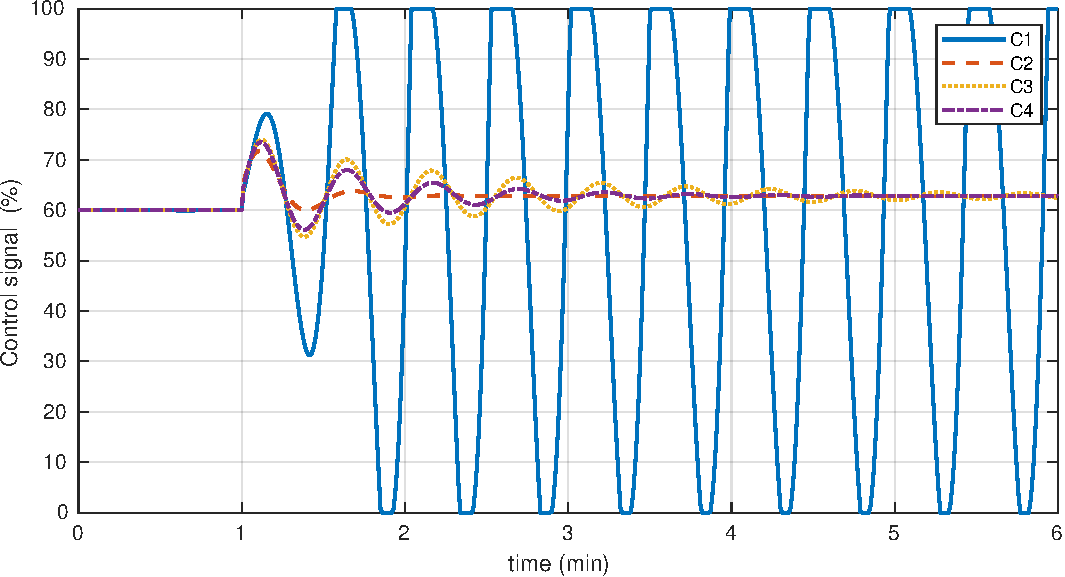
\includegraphics[width=0.8\linewidth]{CH7CSTRControlServoMs10U} \label{fig:CH7CSTRControlServoMs10U}}
	\caption{Control signal of the controlled system with the nonlinear model for several robustness levels serving as servo.}
	\label{fig:CH7CSTRControlServoU}
\end{figure}
%
In Table~\ref{tab:CSTRIAEServo}, the \gls{iae} for the servo response to a step change in the reference at $t= \SI{1}{\second}$ is presented, with the response  plotted in Figure~\ref{fig:CH7CSTRControlServoY}. On the other hand the total variation is presented in Table~\ref{tab:CSTRTVServo} en the control signal in Figure~\ref{fig:CH7CSTRControlServoU}. All controllers where tested for all possible robustness measures.

The first thing to notice is that for the case of $M_s \geq 2.0$, presented in Figure~\ref{fig:CH7CSTRControlServoMs10Y}, the response becomes practically unstable for the C1 tuning. The \gls{pid} controller that was implemented in \simulink have and antiwindup loop that prevents the integral part to become infinite. For the other cases the response presents important oscillations. The problem with C1 is that the gain is relatively high, which produces the controller to saturate as can be seen in Figure~\ref{fig:CH7CSTRControlServoMs10U}.

For this particular case, controller C2 (which was expected to be the ``best'' servo) yield a better \gls{iae} when comparing the $M_s \geq 2.0$ against $M_s = 1.8$ and $M_s = 2.0$ as it was expected knowing Table~\ref{tab:CSTRDesigns}, however this is not the case for C4 controllers, because the nonlinearity of the plant and the approximations made start to take a toll on the design of the controllers.

Now consider the controllers that took into account the robustness as a constraint in the optimization. For all cases the controller are able to control the plant without oscillation (except for controller C1). As expected, controllers C2 and C4 had the best performance, but also the were more expensive (higher values of TV). However, an interesting option is controller C3. This controller was designed by allowing a 20\% degradation of $J_{di}$. Its servo response may not be the best in terms of performance but it has an interesting compromise between the control effort and the \gls{iae} value. If this degradation does not affect the regulator response too much, this controller may be considered as the final tuning.

The next step is then to validate the response as a regulator. %
%
\begin{table}[tb]
	\centering
	\caption{IAE values for the controllers applied to the nonlinear model as regulator controllers}
	\begin{tabular}{p{1.5cm}>{\centering}p{1cm}>{\centering}p{1cm}>{\centering}p{1cm}>{\centering\arraybackslash}p{1cm}}
		\toprule
		\multirow{2}{*}{Robustness}	& \multicolumn{4}{c}{Controller}\\
		\cmidrule{2-5}
		& C1 & C2 & C3 & C4 \\
		\midrule
		$M_s = 1.8$ & 2.29 & 3.40 & 2.54 & 2.85\\
		$M_s = 2.0$ & 2.03 & 3.24 & 2.26 & 2.65\\
		$M_s \geq 2.0$ & 11.62 & 3.18 & 1.97 & 2.00\\
		\bottomrule
	\end{tabular}
	\label{tab:CSTRIAEReg}
\end{table}
%
\begin{table}[tb]
	\centering
	\caption{TV values for the controllers applied to the nonlinear model as regulator controllers}
	\begin{tabular}{p{1.5cm}>{\centering}p{1cm}>{\centering}p{1cm}>{\centering}p{1cm}>{\centering\arraybackslash}p{1cm}}
		\toprule
		\multirow{2}{*}{Robustness}	& \multicolumn{4}{c}{Controller}\\
		\cmidrule{2-5}
		& C1 & C2 & C3 & C4 \\
		\midrule
		$M_s = 1.8$ & 13.30 & 11.85 & 12.50 & 11.65\\
		$M_s = 2.0$ & 13.68 & 15.54 & 13.16 & 14.10\\
		$M_s \geq 2.0$ & 3034.50 & 22.00 & 183.90 & 84.00\\
		\bottomrule
	\end{tabular}
	\label{tab:CSTRTVReg}
\end{table}
%
\begin{figure}
	\centering
	\subfloat[$M_s = 2.0$]{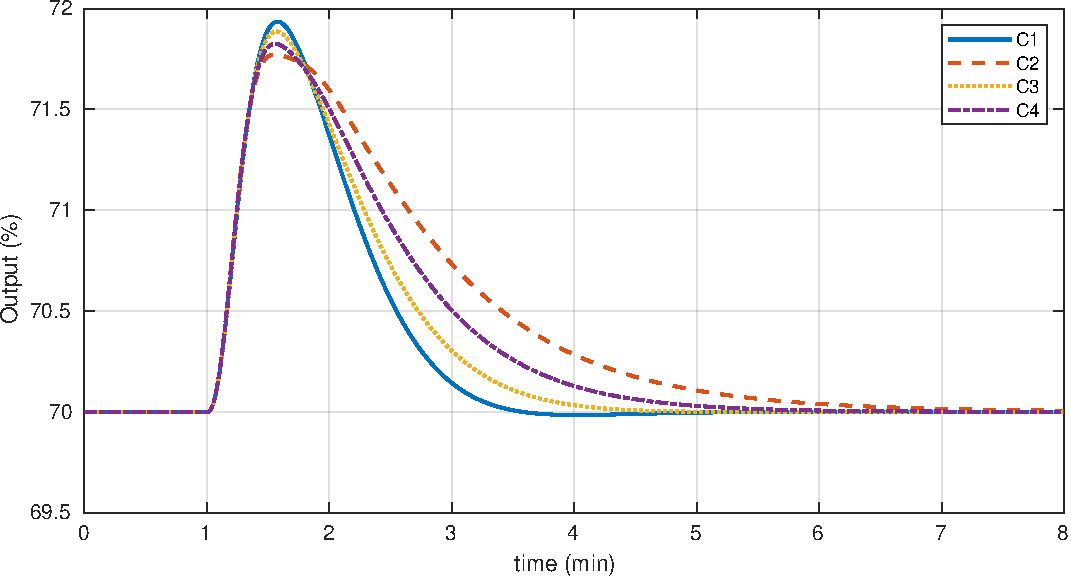
\includegraphics[width=0.8\linewidth]{CH7CSTRControlRegMs2Y} \label{fig:CH7CSTRControlRegMs2Y}}\\
	\subfloat[$M_s = 1.8$]{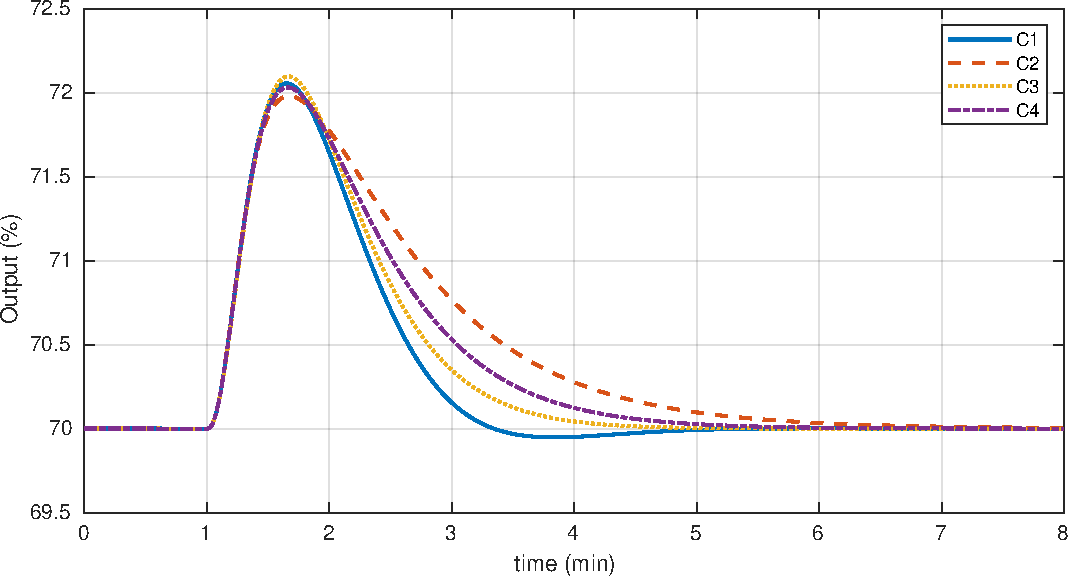
\includegraphics[width=0.8\linewidth]{CH7CSTRControlRegMs18Y} \label{fig:CH7CSTRControlRegMs18Y}}\\
	\subfloat[$M_s \geq 2$]{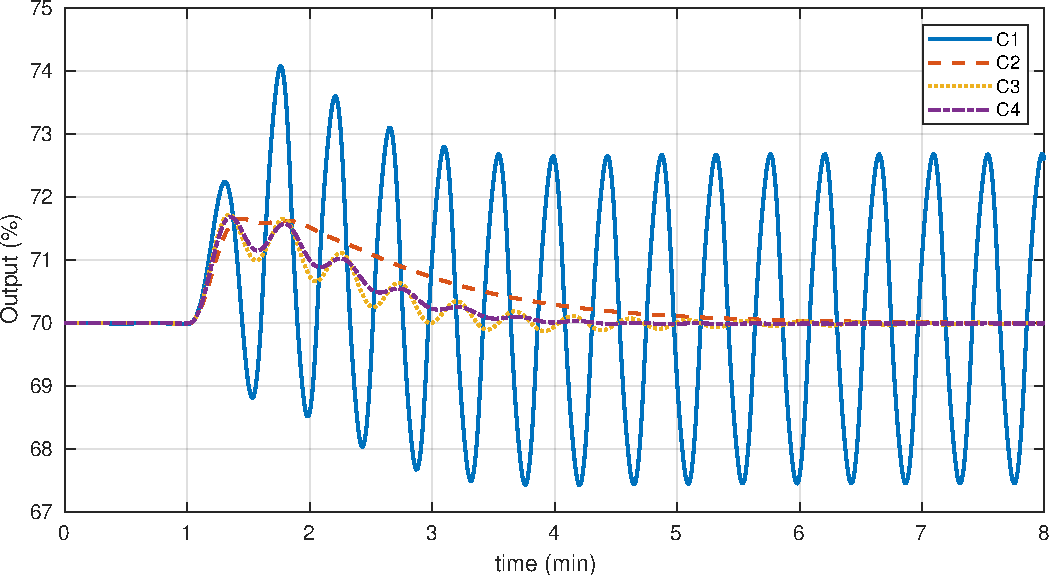
\includegraphics[width=0.8\linewidth]{CH7CSTRControlRegMs10Y} \label{fig:CH7CSTRControlRegMs10Y}}
	\caption{Response of the controlled system with the nonlinear model for several robustness levels serving as regulator.}
	\label{fig:CH7CSTRControlRegY}
\end{figure}
%
%
\begin{figure}
	\centering
	\subfloat[$M_s = 2.0$]{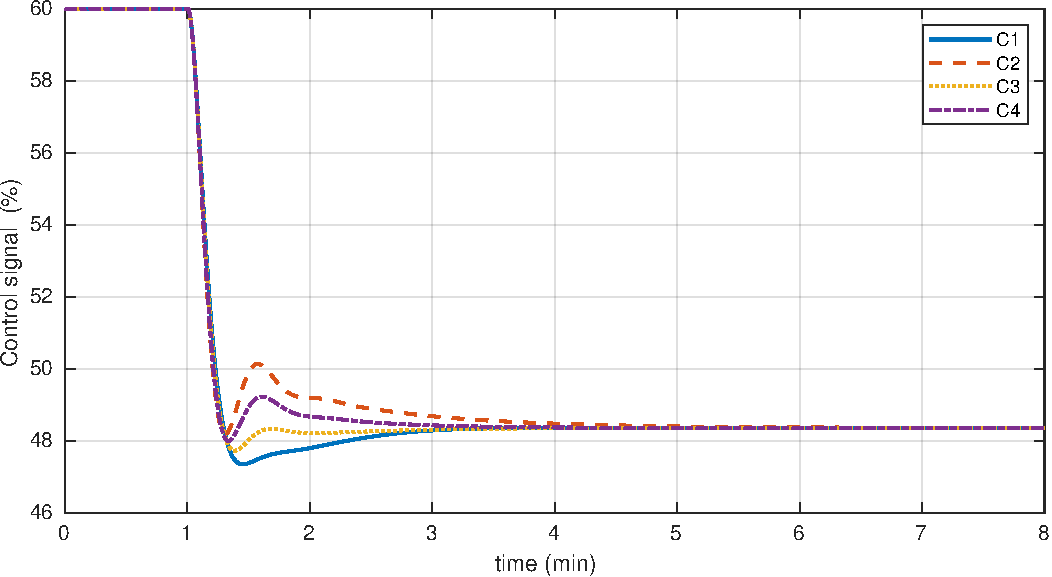
\includegraphics[width=0.8\linewidth]{CH7CSTRControlRegMs2U} \label{fig:CH7CSTRControlRegMs2U}}\\
	\subfloat[$M_s = 1.8$]{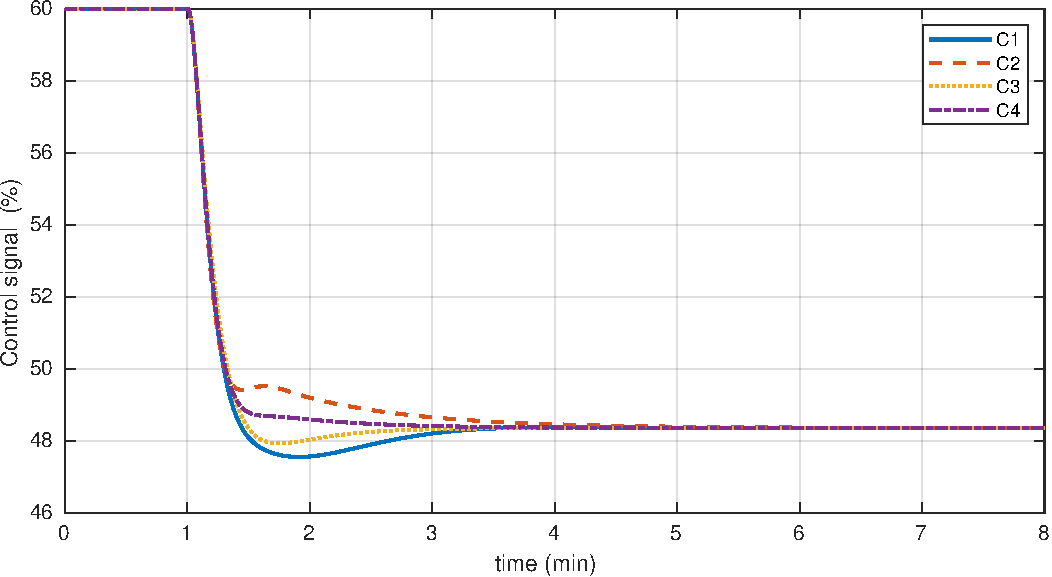
\includegraphics[width=0.8\linewidth]{CH7CSTRControlRegMs18U} \label{fig:CH7CSTRControlRegMs18U}}\\
	\subfloat[$M_s \geq 2$]{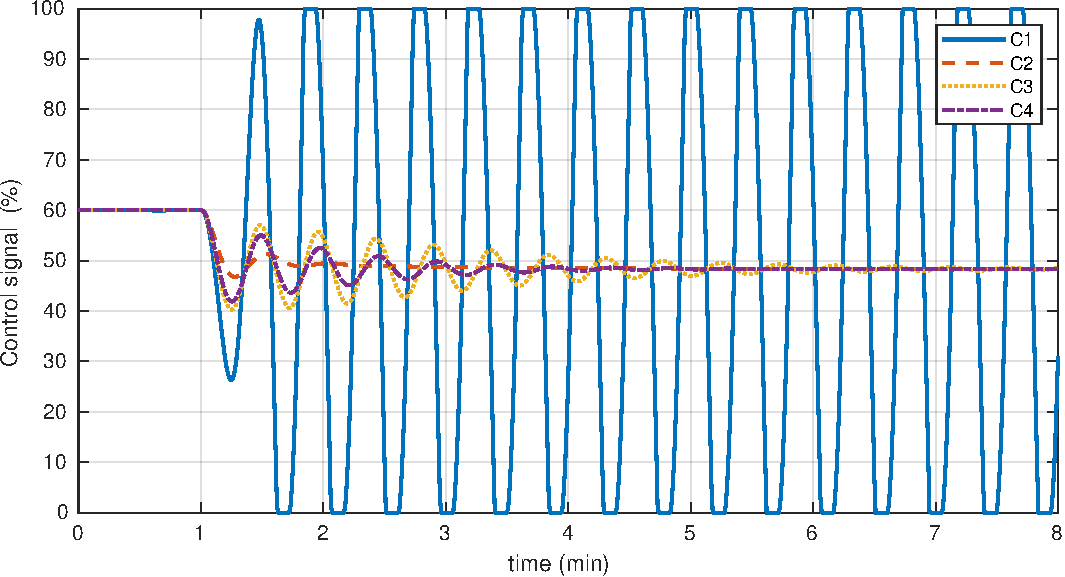
\includegraphics[width=0.8\linewidth]{CH7CSTRControlRegMs10U} \label{fig:CH7CSTRControlRegMs10U}}
	\caption{Control signal of the controlled system with the nonlinear model for several robustness levels serving as regulator.}
	\label{fig:CH7CSTRControlRegU}
\end{figure}
%
Table~\ref{tab:CSTRIAEReg} the values of \gls{iae} are presented for a step change of $\SI{1}{\mole\per\liter}$ in $C_{ai}$ for all controller cases and robustness values. The corresponding values of $TV$ are presented in Table~\ref{tab:CSTRTVReg}. The plots of the responses and the control signal are shown in Figure~\ref{fig:CH7CSTRControlRegY} and Figure~\ref{fig:CH7CSTRControlRegU} respectively. As in the case of the servo response, the design for $M_s \geq 2.0$ is not useful in the C1 case, because the response is practically unstable again as depicted in Figure~\ref{fig:CH7CSTRControlRegMs10Y}. It has to be noticed that the response of the plant between $C_{ai}$ and the output does not have a non-minimum phase zero, and therefore an inverse response is not present.

For the other cases ($M_s = 2.0$ and $M_s = 1.8$) the best controllers were the C1 family, followed by C3. This is expected since these controllers were found as the best regulators. Controller C2 has the worst regulator response but at the same time, it as also the most expensive cost signal for the case $M_s = 2.0$.

Let's examine C3 controllers. The performance of this controllers are worse than C1, but just by approximately 11\%, and with a less aggressive control signal for the regulator response (Table~\ref{tab:CSTRTVReg}). Taking into account that C3 was also a family of controllers that had a relatively good performance for servo control, so far it represents a good candidate to become the final controller.

As a final validation test, let the setpoint change to be 5\%. In that case the response is as given in %
%
\begin{figure}[tb]
	\centering
	\subfloat[Output signal]{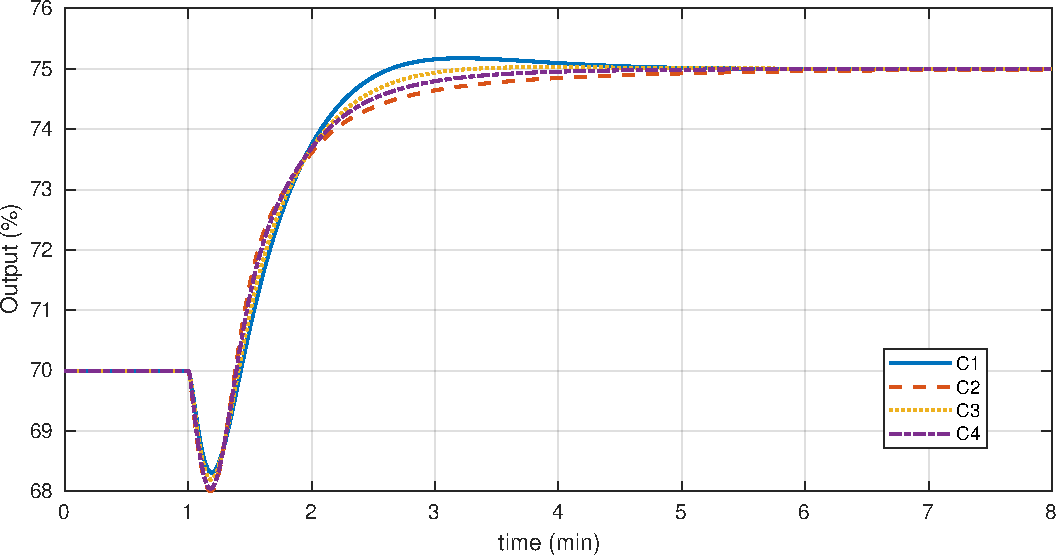
\includegraphics[width=\linewidth]{CH7CSTRControlServoMs2Y_Sat}\label{fig:CH7CSTRControlServoMs2Y_Sat}}\\
		\subfloat[Control signal]{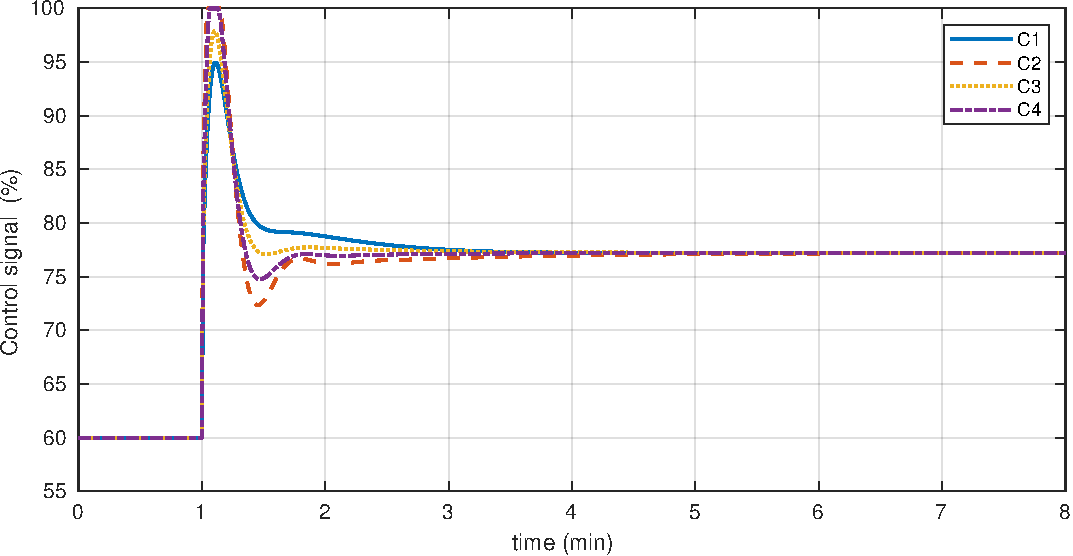
\includegraphics[width=\linewidth]{CH7CSTRControlServoMs2U_Sat}\label{fig:CH7CSTRControlServoMs2U_Sat}}
	\caption{Response to a 5\% step change in the setpoint signal.}
	\label{fig:CH7CSTRControlServoSat}
\end{figure}
%
Figure~\ref{fig:CH7CSTRControlServoSat} for all controllers families and $M_s = 2.0$.
%
\begin{table}[tb]
	\centering
	\caption{IAE values for the controllers applied to the nonlinear model as servo controller for a step change of 5\% and $M_s = 2.0$}
	\begin{tabular}{c>{\centering}p{1cm}>{\centering}p{1cm}>{\centering}p{1cm}>{\centering\arraybackslash}p{1cm}}
		\toprule
		\multirow{2}{*}{Cost function}	& \multicolumn{4}{c}{Controller}\\
		\cmidrule{2-5}
		& C1 & C2 & C3 & C4 \\
		\midrule
		IAE & 4.69 & 5.07 & 4.60 & 4.71\\
		TV	& 52.70	& 73.44	& 59.81	& 68.01\\
		\bottomrule
	\end{tabular}
	\label{tab:CSTRIAEServoSat}
\end{table}
%

The values of IAE and TV are presented in Table~\ref{tab:CSTRIAEServoSat}. The PID was implemented to be limited in the range between 0 and 100\%, with the corresponding antiwindup. Since controllers C2 and C4 have a control signal which is more aggressive for setpoint changes, they saturate and produces larger values of IAE than the controllers intended for regulation. Interestingly, C3 controller has a lower value of IAE than any other controller while its TV value lies in between C1 and C4 controllers. Again, this test indicates that C3 controller can be a good candidate for the final tuning of the \gls{pid}.

Lastly, lets again set the change in the setpoint to 5\%, but lets compare the difference when C3 is selected as the controller and the $M_s$ is varied. %
%
\begin{figure}[tb]
	\centering
	\subfloat[Output signal]{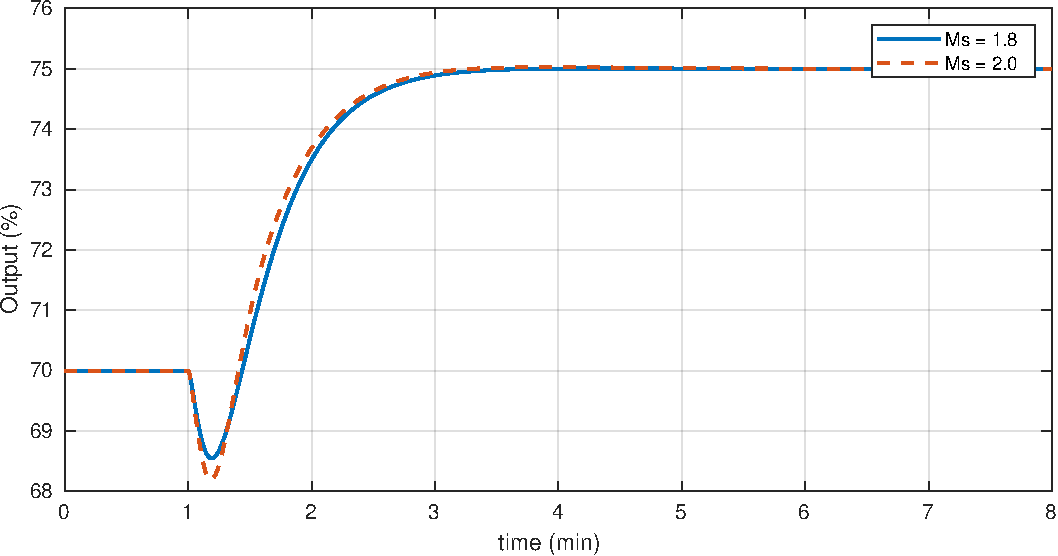
\includegraphics[width=\linewidth]{CH7CSTRControlServoC3Y_Sat}\label{fig:CH7CSTRControlServoC3Y_Sat}}\\
	\subfloat[Control signal]{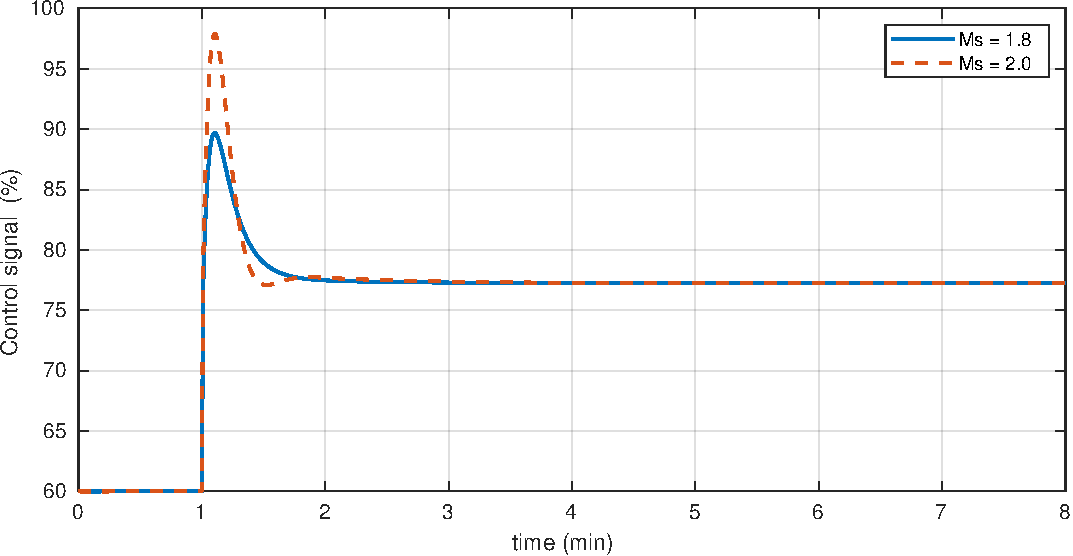
\includegraphics[width=\linewidth]{CH7CSTRControlServoC3U_Sat}\label{fig:CH7CSTRControlServoC3U_Sat}}
	\caption{Response to a 5\% step change in the setpoint signal for C3 controllers.}
	\label{fig:CH7CSTRControlServoC3Sat}
\end{figure}
%
\begin{table}[tb]
	\centering
	\caption{IAE values for the C3 controllers applied to the nonlinear model as servo controller for a step change of 5\%}
	\begin{tabular}{c >{\centering}p{1cm}>{\centering\arraybackslash}p{1cm}}
		\toprule
		\multirow{2}{*}{Cost function}	& \multicolumn{2}{c}{$M_s$}\\
		\cmidrule{2-3}
		& 1.8 & 2.0 \\
		\midrule
		IAE & 4.83 & 4.61 \\
		TV	& 42.11	& 59.81	\\
		\bottomrule
	\end{tabular}
	\label{tab:CSTRIAEServoC3Sat}
\end{table}
%
In Figure~\ref{fig:CH7CSTRControlServoC3Sat} the output of the controlled loop and the control signal is presented and in Table~\ref{tab:CSTRIAEServoC3Sat}, the values of IAE and TV are presented for both $M_s = 1.8$ and $M_s = 2.0$. As it was expected, since neither of those controllers saturates, the response with a less restrictive robustness constraint has a better IAE. However it certainly has a more aggressive control signal. The IAE for the case $M_s = 2.0$ is $4.55\%$ lower than the $M_s = 1.8$ case however it comes to a cost of having a $42.03\%$ higher TV. Considering all the analysis done to this point and having into account that the tuning were made with an several approximations from the original model, it seem that the C3 tuning (best servo allowing a 20\% degradation on $J_{di}$) with a robustness constraint of $M_s = 1.8$ is the most sensible choice as the final tuning.
%\cite{Kuntanapreeda2012}
 
\section{Final remarks}
\label{sec:FinalRemarks}
The motivation of the examples presented in this chapter was to show all the advantages that can be derived from using a multiobjetive approach when tuning a PID controller for industrial applications. As it was shown, the final selection of the parameters was defined not only by its optimal value, but also, according to the robustness needs and the level of compromise between the cost functions.

However, it has to be noticed that the cost function selected for these studies are totally  arbitrary and other authors may choose to optimize the tuning of the parameters with other criteria. For example, in Section~\ref{sec:ParetoPractical}, the total variation was selected as one of the cost functions and the Pareto found was considerably different than the ones found using $J_{di}$, $J_{do}$ and $J_r$. But it is known that the \gls{iae} is a practical measure on the optimality of the control in industry \citep{Shinskey2002}, and for this reason was the selected cost function for the tool presented in this book and consequently the examples examined in this chapter.

Apart from the theoretical contribution of this book, the \matlab tool that is included along with the complete set of data, represents an interesting starting point for further studies. Of course the methodology presented in \ref{sec:SolMOOP} is completely general and can (and is encouraged) to be change to the needs of the decision maker.

One of the most interesting characteristics of control systems is that it always implies some kind of compromise. The relationship between servo and regulation control, or between performance and aggressiveness is always something that has to be taken into account along with the need to have a robust control system that is able to keep working despite the difference between the model and the actual plant. It is the desire of the authors to have helped in the development of a deeper understanding on this issues, and to open the door to more research in the field of optimization applied to industrial control.

\bibliographystyle{spbasic}
\bibliography{ReferenciasMulti}